% $Id: anleitung.tex,v 1.19 2009/05/31 04:57:01 baum Exp $
% Tag $Name: tinyheb-1-6-3 $

% Copyright (C) 2004 - 2013 Thomas Baum <thomas.baum@arcor.de>
% Thomas Baum, 42719 Solingen, Germany

% This program is free software; you can redistribute it and/or modify
% it under the terms of the GNU General Public License as published by
% the Free Software Foundation; either version 2 of the License, or
% (at your option) any later version.

% This program is distributed in the hope that it will be useful,
% but WITHOUT ANY WARRANTY; without even the implied warranty of
% MERCHANTABILITY or FITNESS FOR A PARTICULAR PURPOSE.  See the
% GNU General Public License for more details.

% You should have received a copy of the GNU General Public License
% along with this program; if not, write to the Free Software
% Foundation, Inc., 59 Temple Place - Suite 330, Boston, MA 02111-1307, USA.


\chapter {Anleitung\label{anleitung}}
In diesem Kapitel ist die komplette Anleitung zu \tinyHeb\/ beschrieben. Zunächst wird auf die Erfassung von Stammdaten eingegangen, inkl. einer Übersicht 
welche Plausibilitäten Prüfungen für die einzelnen Felder hinterlegt sind.
Im Abschnitt Rechnungserfassung werden die Besonderheiten bei der
Erfassung der Rechnung aufgezeigt. Es wird insbesondere beschrieben, welche
Rechnungsposten in welchen Fällen automatisch ermittelt werden. Es werden
aber auch die Grenzen des Programms gezeigt, d.h. an welchen Stellen muss
die Anwenderin selbst darauf achten, dass z.B. Zuschläge richtig erfasst
werden.

\section{Stammdatenerfassung\label{stammdatenerfassung:kap}}
\index{Stammdaten}
\index{Patientinnen|see{Stammdaten}}
In diesem Abschnitt werden alle Felder beschrieben, die erfasst werden
können und welche Auswirkung diese in der späteren Be-/ Verarbeitung haben.
Es wird gezeigt, wie ``Frauen'' angelegt, geändert,
respektive gelöscht werden können und
welche Funktionen die einzelnen Knöpfe auf der Maske haben.\par
Über den Link \verb|Stammdaten| gelangt man aus dem Hauptmenue 
(Abbildung \vref{einstieg:fig}) in die Maske Stammdaten
(siehe Abbildung \vref{stammdatenerfassung:fig}).

\begin{figure}[ht]
\centering
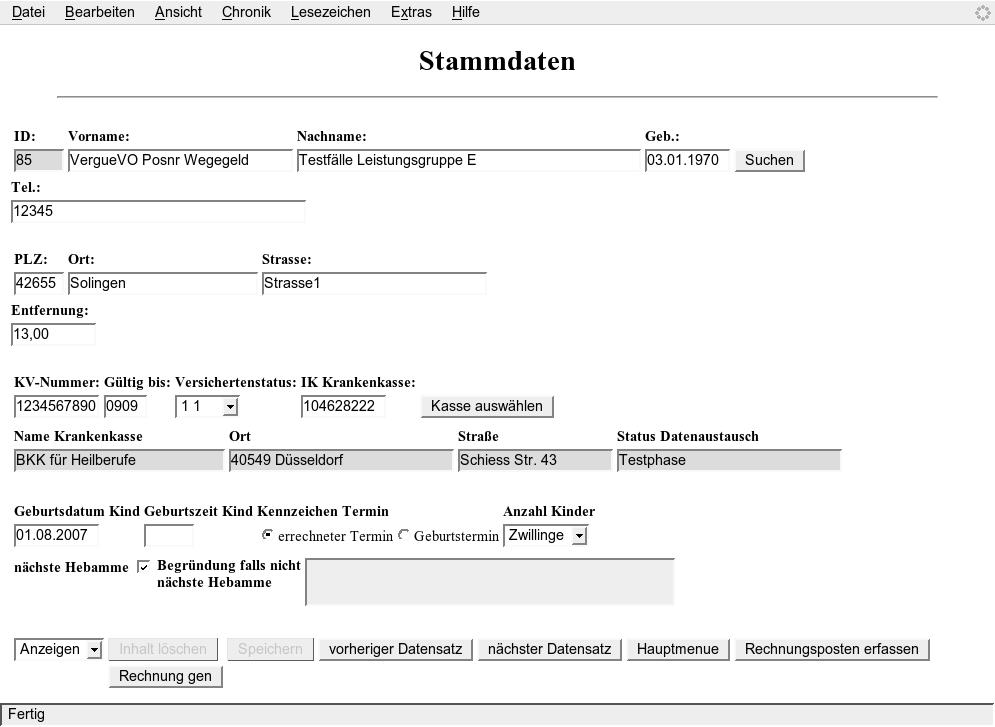
\includegraphics[width=9cm]{stammdaten}
\caption{Stammdatenerfassungsmaske\label{stammdatenerfassung:fig}}
\end{figure}

\subsection{Beschreibung der Stammdatenfelder}
Der Cursor steht nach Aufruf der Maske immer im ersten leeren  Feld.
Bei einer leeren Maske also im Feld \feld{Vorname}.
Folgende Felder sind auf der Maske vorhanden:
\begin{description}
\item[ID] Dieses Feld enthält die interne ID zum angezeigten Datensatz,
es wird automatisch gefüllt und kann nicht erfasst oder geändert werden.
\item[Vorname] Dieses Feld enthält den Vornamen der Frau, es können maximal 30 Zeichen erfasst werden\footnote{im Rahmen des elektronischen Datenaustausches sind für den Vornamen nur 30 Zeichen vorgesehen}. Der Vorname wird in die spätere Rechnung übernommen.
Eine Prüfung ob der Vorname erfasst wird, existiert an dieser Stelle nicht.
\item[Nachname] Das Feld enthält den Nachnamen der Frau, es können maximal 47 Zeichen erfasst werden\footnote{im Rahmen des elektronischen Datenaustausches sind für den Nachnamen nur 47 Zeichen vorgesehen}. Der Nachname wird in die spätere Rechnung übernommen.
Eine Prüfung ob der Nachname erfasst wird, existiert an dieser Stelle nicht.
\item[Geb.] Dieses Feld enthält das Geburtsdatum der Frau. Das Datum wird
in die spätere Rechnng übernommen. Die Erfassung muss
im Format TT.MM.JJJJ oder TT.MM.JJ erfolgen. 
Wird das Datum im Format TT.MM.JJ erfasst, erfolgt nach Verlassen des
Feldes automatisch die Ermittlung und Darstellung der 4-stelligen Jahreszahl.
Ein ungültiges Datum führt zu der Fehlermeldung: Bitte gültiges Datum erfassen.
Das Speichern des Formulares mit ungültigen Werten ist nicht möglich.
\item[Tel.] Das Feld enthält die Telefonnummer der Frau, es können beliebige
Zeichen erfasst werden. Das Feld hat rein informativen Charakter 
und wird in der weiteren Anwendung
nicht mehr verwendet\footnote{dies kann sich zukünftig ändern, z.B. bei
Auswertungen oder Listen, die produziert werden, Stand 04.09.2005}.
\item[PLZ] Das Feld enthält die PLZ zur Anschrift der Frau. Es wird in die 
spätere Rechnung übernommen. Es muss eine 5-stellige numerische Zahl
 erfasst werden. Das
bedeutet, eine 4-stellige PLZ, wie z.B. 04177 Leipzig,
muss mit führender Null erfasst werden. Ob
die PLZ im Sinne der Post wirklich gültig ist oder nicht, wird nicht
geprüft. Ein nicht korrekter Wert führt zu einer entsprechenden Fehlermeldung,
die durch Drücken des Knopfes \knopf{OK} bestätigt werden muss.
Das Speichern des Formulares mit ungültigen Werten ist nicht möglich (siehe auch Feld Geb.).
Eine Prüfung, ob die PLZ erfasst wird, existiert an dieser Stelle nicht.
\item[Ort] Das Feld enthält den Ort zur Anschrift der Frau, es können
maximal 25 Zeichen erfasst werden. Der Ort wird in die 
spätere Rechnung übernommen. Eine Prüfung, ob der Ort erfasst wird, exisiert
an dieser Stelle nicht.
\item[Strasse] Das Feld enthält die Strasse zur Anschrift der Frau, es können
maximal 30 Zeichen erfasst werden. Die Strasse wird in die 
spätere Rechnung übernommen. Eine Prüfung, ob die Strasse erfasst wird, 
exisiert an dieser Stelle nicht.
\item[Entfernung] Das Feld enthält die Entfernung von der Hebamme bis zur Frau.
Der Inhalt wird in die Maske Rechnungsposten erfassen übernommmen.
\item[KV-Nummer] Das Feld enthält die Krankenversicherungsnummer der Frau, die
in die spätere Rechnung übernommen wird.
Es muss 9 oder 10-stellig numerisch erfasst werden. 
Das bedeutet, es muss ggf. mit
führenden Nullen erfasst werden. Ein nicht korrekter Wert führt zu einer
entsprechenden Fehlermeldung, die durch Drücken des Knopfes \knopf{OK}
bestätigt werden muss (analog dem Feld PLZ). Eine Prüfung, ob die KV-Nummer
erfasst wird, existiert an dieser Stelle nicht.
\item[Gültig bis] Das Feld enthält die Gültigkeitsdauer der Versichertenkarte
der Frau und wird in die spätere Rechnung übernommen. Es muss im Format
MMJJ erfasst werden. Die Fehlerbehandlung erfolgt analog den Feldern
PLZ und KV-Nummer. Eine Prüfung, ob das Feld erfasst wird, existiert an
dieser Stelle nicht,
\item[Versichertenstatus] 
\index{Versichertenstatus}
Das Feld enthält den Versichertenstatus der Frau
und wird in die spätere Rechnung übernommen. Per Pop Down Menue können
die Werte '1 1', '3 1', 'privat', '1 9', '3 9','1 7','3 7','1 8','3 8','5 1',
'5 9','SOZ' ausgewählt werden.
\item[IK Krankenkasse] Das Feld enthält die IK Nummer der Krankenkasse der
Frau und wird in die spätere Rechnung übernommen. Anhand der IK Nummer
wird der Name und die Rechnungsanschrift der Krankenkasse ermittelt. Ohne
die Angabe der IK Nummer kann keine ordnungsgemäße Rechnung produziert werden.
Die Nummer ist 9-stellig numerisch zu erfassen. Wird das Feld nur 7-stellig
numerisch erfasst, wird automatisch 10 vorangestellt, da in der Regel
die IK Nummer nur 7-stellig auf der Versichertenkarte angegeben ist.
Die Vorgehensweise bzgl.
der Fehlerkorrektur ist analog zu den Feldern \feld{PLZ} und \feld{Geb.}
\item[Name der Krankenkasse, Ort, Straße, Status Datenaustausch] 
Diese Felder enthalten die 
Anschrift der Krankenkasse sowie den Status zum Datenaustausch
und können nicht erfasst werden. Die Werte werden
anhand der IK Nummer der Krankenkasse automatisch nach dem Speichern
gefüllt. Wurde im Feld \feld{IK Krankenkasse} eine unbekannte IK Nummer
erfasst, erscheint im Feld \feld{Name der Krankenkasse} der Hinweistext:
``nicht bekannte IK angegeben''. Wurde im Feld \feld{Versichertenstatus} privat
ausgewählt, wird der Hinweistext: ``Privat versichert'' ausgegeben.
Im Feld \feld{Status Datenaustausch} ist angegeben in welchem Status mit dieser
Krankenkasse der Datenaustausch abgewickelt wird. Mögliche Werte sind:
\begin{enumerate}
\item 
kein elektronischer Datenaustausch
\item 
Testphase
\item
Erprobungsphase
\item
Echtbetrieb
\end{enumerate}
\item[Geburtsdatum Kind] Dieses Feld enthält das Geburtsdatum, bzw. den
errechneten Geburtstermin des Kindes und wird in die spätere Rechnung 
übernommen. 
Anhand dieses Feldes werden u.a.
Materialpauschalen bei der Erfassung von Rechnungsposten ermittelt.
Die Plausiprüfungen erfolgen analog dem Feld \feld{Geb.} Eine Prüfung,
ob das Geburtsdatum Kind erfasst wird, existiert nicht.
\item[Geburtszeit Kind]
In diesem Feld muss die Uhrzeit der Geburt erfasst werden. Es kann frei
gelassen werden, wenn es sich bei dem Geburtsdatum um den errechneten
Termin handelt oder die Uhrzeit nicht bekannt ist. 
Das Feld muss im Format HH:MM erfasst werden.
Ein nicht korrekter Wert führt zu einer entsprechenden Fehlermeldung,
die durch Drücken des Knopfes \knopf{OK} bestätigt werden muss.
Das Speichern des Formulares mit ungültigen Werten ist nicht möglich.
\footnote{Dieses Feld wird ab dem 01.02.2008 in die elektronische
Rechnung übernommen.}
\item[Kennzeichen Termin]
Über diesen Schalter wird gesteuert, ob es sich im Feld 
\feld{Geburtsdatum Kind}
um das Geburtsdatum,  bzw. den errechneten Geburtstermin des Kindes
handelt. Wird Geburtstermin angegeben, wird auf der Rechnung ``geboren am'' 
angedruckt, sonst wird ``ET'' angedruckt.
\footnote{Dieses Feld wird ab dem 01.02.2008 in die elektronische
Rechnung übernommen.}
\item[Anzahl Kinder] Das Feld enthält die Anzahl der Kinder, die bei dem
Geburtsdatum angegebenen Termin zur Welt gebracht wurden. Sind mehrere
Kinder zur Welt gekommen, wird dies auf der späteren Rechnung ausgewiesen.
Per Pop Down Menue können bis zu vier Kinder ausgewählt werden.
\item[nächste Hebamme] Dieses Feld enthält einen Schalter, ob die Hebamme,
die nächste Hebamme ist. Das Feld hat rein informativen Charakter. Ist der
Schalter angekreuzt, ist das Feld \feld{Begründung falls nicht nächste
Hebamme} für die Erfassung gesperrt.
\item[Begründung falls nicht nächste Hebamme] Dieses Feld kann eine frei
formulierte Begründung enthalten, falls die Hebamme nicht die nächste Hebamme
ist. Das Feld hat rein informativen Charakter und wird in der weitere
Anwendung nicht verwendet. Eine Erfassung ist nur möglich, wenn der Schalter
\feld{nächste Hebamme} nicht gesetzt ist.
\end{description}
Erst bei der Rechnungserstellung wird geprüft, ob die Felder
\feld{Vorname, Nachname, Geburtsdatum Frau, Geburtsdatum Kind, KV-Nummer, Versichertenstatus, Geburtszeit Kind,
IK-Krankenkasse} gefüllt sind. Ist dies nicht der Fall, kann keine
Rechnung erstellt werden. Wobei die Felder \feld{KV-Nummer} und 
\feld{IK-Krankenkasse}
nur dann notwendig sind, wenn es sich um eine Kassenrechnung handelt.
Im Kapitel \vref{rechnungsgenerierung:kap} sind die Prüfungen im Detail
beschrieben.

\subsection{Beschreibung der Knöpfe im Stammdatenmenue}
\begin{description}
\item[Suchen] 
Mit dem Knopf \knopf{Suchen} kann eine weitere Maske geöffnet
werden, über die Frauen gesucht werden können. Die Beschreibung zu der
Suchmaske befindet sich in Abschnitt \vref{frauenauswahl:abs}.
In diese Maske werden die Werte aus den Feldern \feld{Vorname, Nachname}
sowie
\feld{Geb.} übernommen und die Suche unmittelbar gestartet.
\item[Kasse auswählen] 
Mit dem Knopf \knopf{Kasse auswählen} wird ein Maske
geöffnet, über die Krankenkassen gesucht werden können. Die Beschreibung zu
der Suchmaske befindet sich in Abschnitt \vref{kassenauswahl:abs}. Eine
Übernahme von Daten, wie beim Knopf \knopf{Suchen} erfolgt nicht.
\item[Inhalt löschen] 
Der Knopf \knopf{Inhalt löschen} ist nur dann Aktiv, wenn in dem
Pop Down Menue vor dem Knopf der Wert Neu ausgewählt wurde. Wird der Knopf
gedrückt, werden die Feldinhalte aller Felder der Maske gelöscht und das
Pop Down Menue springt auf den Wert Anzeigen. Der Datensatz selbst wird
nicht gelöscht.
\item[Speichern/ Löschen] Der Knopf \knopf{Speichern} ist nur dann aktiv,
wenn im
Auswahlmenue entweder der Wert Neu oder Ändern gewählt wird. 
\par
Falls \knopf{Neu}
ausgewählt wurde, wird ein neuer Kundinnensatz in der Datenbank gespeichert
und das Pop Down Menue springt auf den Wert Anzeigen. Neben den oben
beschriebenen Plausibilitäten Prüfungen findet beim Speichern keine weitere
Prüfung statt.\par
Falls \knopf{Ändern} gewählt wurde, wird der Datensatz, der sich in der Datenbank
befindet mit den angezeigten Werten überschrieben und das Pop Down Menue
springt auf den Wert Anzeigen. Neben den oben beschriebenen
Plausibilitätenprüfungen finden keine weiteren Prüfungen statt.

Falls im Pop Down Menue \knopf{Löschen} ausgewählt wurde, erhält der Knopf die
Beschriftung Löschen. Durch Drücken des Knopfes wird der Datensatz aus der
Datenbank gelöscht. Es wird bei der Löschung geprüft, ob schon Leistungen
erfasst wurden. Ist dies der Fall, kann der Datensatz nicht mehr gelöscht 
werden und es erscheint die Fehlermeldung ``Löschen nicht möglich, es sind
schon Leistungen erfasst''. Wurde der Datensatz erfolgreich gelöscht, werden
alle Feldinhalte der Felder der Maske gelöscht und das Auswahlmenue
steht auf den Wert Anzeigen. Konnte der Datensatz nicht gelöscht werden,
bleiben die Inhalte der Felder erhalten. Das Auswahlmenue springt auf den 
Wert Anzeigen.
\item[vorheriger Datensatz] Dieser Knopf ist nur dann aktiv, wenn der Wert
des Pop Down Menues auf Anzeigen steht. Durch Drücken des Knopfes wird auf
den vorherigen Datensatz in der Datenbank gesprungen. Der vorherige Datensatz
ist derjenige, mit der nächst kleineren ID, als die im Feld \feld{ID}
angezeigte. Ist
man am ersten Datensatz angekommen, bleibt dieser in der Maske erhalten.
\item[nächster Datensatz] Dieser Knopf ist nur dann aktiv, wenn der Wert
des Pop Down Menues auf Anzeigen steht. Durch Drücken des Knopfes wird auf
den nächsten Datensatz in der Datenbank gesprungen. Der nächste Datensatz
ist derjenige, mit der nächst höheren ID, als die im Feld \feld{ID}
 aktuell angezeigte. Ist
man am letzten Datensatz angekommen, bleibt dieser in der Maske erhalten.
\item[Hauptmenue] Über diesen Knopf gelangt man in das Hauptmenue.
Dabei ist zu beachten, dass nicht überprüft wird, ob Änderungen oder Neu
erfasste Daten gespeichert wurden. Es wird sofort in die Maske Hauptmenue
gesprungen.
\item[Rechnungsposten erfassen] Über diesen Knopf gelangt man in die Maske
zur Erfassung von Rechnungsposten. Ein Sprung in die Maske ist nur 
möglich, wenn eine Kundin und \knopf{Anzeigen} ausgewählt ist. Die 
Stammdaten der Kundin werden in die Maske Rechnungsposten erfassen übernommen.
\item[Rechnung gen] Über diesen Knopf gelangt man in die Maske zum Ausdruck
der noch in Bearbeitung befindlichen Rechnungsposten. Ein Sprung in die Maske
ist nur dann möglich, wenn eine Kundin und \knopf{Anzeigen} gewählt ist. Die
Stammdaten der Kundin werden in die Maske Rechnungsgenerierung übernommen.
\end{description}

Sind alle Felder erfasst, müssen die Daten gespeichert werden. Dazu ist
es notwendig im Pop Down Menue unten links den Wert 'Neu' auszuwählen.
Sobald dies geschehen ist, wird der Knopf \knopf{Speichern} aktiv 
geschaltet. Drückt man jetzt den Knopf \knopf{Speichern} werden die Daten
zu der Frau permanent abgelegt. Nach dem Speichern wird die Auswahl im 
Pop Down Menue unten links auf den Wert 'Anzeigen' gesetzt.




\section{Frauenauswahl}\label{frauenauswahl:abs}
In diesem Absatz ist beschrieben, wie Kundinnen im Datenbestand gesucht und
ausgewählt werden können.
In der Regel erfolgt der  Aufruf der Maske aus der 
Stammdatenerfassungsmaske (siehe
Seite \pageref{stammdatenerfassung:fig}) 
über den Knopf \knopf{Suchen}. Analoge Knöpfe findet man in dem Masken der
Rechnungspostenerfassung (siehe Seite \pageref{rechnungspostenerfassen:fig})
und der
Rechnungsgenerierung (siehe Seite \pageref{rechnungsgenerierung:fig}).
Klickt man auf den Knopf \knopf{Suchen} wird ein neues Fenster mit der
Überschrift ``Frau suchen'' geöffnet\footnote{sollte das Fenster 
noch geöffnet sein, wird es in den 
Vordergrund des Bildschirms geholt.} 
(siehe Abbildung \vref{frauenauswahl:fig}). Über die Felder \feld{Vorname,
Nachname, Geb. Frau, Geb. Kind, PLZ, Ort und Strasse} ist es möglich die
Suchkriterien vorzugeben, d.h. es werden bei der Suche nur die Frauen
ausgegeben, bei denen alle vorgegebenen Werte vorhanden sind. Dabei ist
folgendes für die Felder zu beachten:

\begin{figure}[h]
\centering
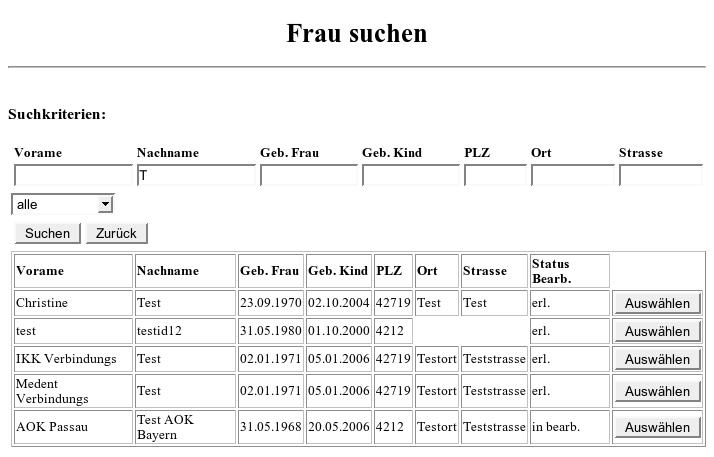
\includegraphics[width=9cm]{frauenauswahl}
\caption{Frauenauswahlmaske\label{frauenauswahl:fig}}
\end{figure}

\begin{description}
\item[Vorname] Es wird nur nach den Frauen gesucht, bei denen der Vorname 
einen Teil des Feldes enthält.
Wird z.B. im Feld \feld{Vorname} ``Maria'' erfasst,
würde Maria Luise und Anna Maria ermittelt werden.
\item[Nachname] Es wird nur nach den Frauen gesucht, bei denen der Nachname mit
dem Feldinhalt beginnt. Wird z.B. im Feld \feld{Nachname} ``D'' erfasst,
würden alle Frauen deren Nachname mit ``D'' beginnt ermittelt werden.
\item[Geb. Frau] Es wird nur nach den Frauen gesucht, die an diesem Tag geboren
sind. Das Feld ist im Format TT.MM.JJJJ zu erfassen, die Plausiprüfungen sind
analog der Prüfungen, die im Kapitel Stammdatenerfassung 
(Seite \pageref{stammdatenerfassung:kap}) beschrieben sind.
\item[Geb. Kind] Es wird nur nach den Frauen gesucht, deren Kinder
an diesem Tag geboren wurden.
Das Feld ist im Format TT.MM.JJJJ zu erfassen, die Plausiprüfungen sind
analog der Prüfungen, die im Kapitel Stammdatenerfassung 
(Seite \pageref{stammdatenerfassung:kap}) beschrieben sind.
\item[PLZ] Es wird nur nach den Frauen gesucht, deren Adresse die im Feld
\feld{PLZ} erfasste PLZ exakt enthält. Die Plausiprüfungen sind analog
der Prüfungen, die im Kapitel Stammdatenerfassung (Seite 
\pageref{stammdatenerfassung:kap}) beschrieben sind.
\item[Ort] Es wird nur nach den Frauen gesucht, bei denen der Ort einen
Teil des Feldes enthält. Wird z.B. im Feld \feld{Ort} ``ing'' erfasst,
würden Frauen an den Orten Sol\textbf{ing}en und Emmend\textbf{ing}en ermittelt.
\item[Strasse] Es wird nur nach den Frauen gesucht, bei denen die Straße einen
Teil des Feldes enthält. Wird z.B. im Feld \feld{Strasse} ``el'' erfasst,
würden alle Frauen die in den Straßen D\textbf{el}ler Str. und 
Ohligser F\textbf{el}d ermittelt.
\end{description}

Über das Auswahlfeld über
dem Knopf \knopf{Suchen} lässt sich die Suche zusätzlich einschränken auf alle
Frauen bei denen Positionen existieren, die in einem Status ungleich
erledigt sind.
Ist der Aufruf der Maske aus der Stammdatenerfassung
erfolgt, werden die Werte Vorname, Nachname sowie das Geburtsdatum der Frau
in die Suchkriterien übernommen und die Suche wird unmittelbar gestartet.
Die Felder können jederzeit mit neuen Suchkriterien gefüllt und die Suche
über den Knopf \knopf{Suchen} gestartet werden.

Das Ergebnis der Suche wird unmittelbar unter den Suchkriterien ausgegeben.
Neben den Daten zu Name und Anschrift wird auch der Bearbeitungsstatus
angezeigt, folgende Status sind möglich:
\begin{description}
\item[in bearb.] 
Es sind keine oder Rechnungsposten erfasst, für die noch
keine Rechnung erstellt wurde.
\item[Rechnung] 
Es wurde eine Papierrechnung erstellt. Es sind keine weiteren
Rechnungsposten vorhanden, für die noch eine Rechnung erstellt werden muss.
\item[Edi Rech.] 
Es wurde eine elektronische Rechnung erstellt. Es sind
keine weiteren Rechnungsposten vorhanden, für die noch eine Rechnung
erstellt werden muss.
\item[Teilzahl.] 
Es wurde für eine Rechnung eine Teilzahlung geleistet. Es
ist weder eine weitere Rechnung vorhanden, für die noch keine Zahlung erfolgt
ist, noch sind weitere Rechnungsposten vorhanden, für die noch eine Rechnung erstellt werden muss.
\item[Mahnung] 
Es wurde für eine Rechnung bereits eine Mahnung erstellt, 
dabei wird angegeben, wie viele Mahnung bisher erstellt wurden.
\item[erl.] 
Es sind weder offene Rechnungsposten noch Rechnungen vorhanden.
\end{description}

Über den Knopf \knopf{Auswählen} werden die Daten der Frau in die Maske
übernommen, aus der die Suchfunktion aufgerufen wurde. Die Maske ``Frau Suchen''
wird danach geschlossen.

Falls keine Frau den gewünschten Suchkriterien entspricht, kann entweder
durch Klicken des Knopfes \knopf{Zurück} die Maske ``Frau Suchen''
geschlossen werden, oder es können andere Suchkriterien erfasst werden.





\section{Krankenkassen\label{krankenkassenerfassung:kap}}
\index{Krankenkassen}
In diesem Abschnitt werden alle Felder beschrieben, die erfasst werden
können und welche Auswirkung diese in der späteren Be-/ Verarbeitung haben.
Es wird gezeigt, wie über die Maske ``Krankenkassen'' angelegt, geändert,
respektive gelöscht werden können und
welche Funktionen die einzelnen Knöpfe in der Maske haben. In der Regel
sollte die manuelle Erfassung von Krankenkassen nicht notwendig sein,
da die aktuellen Daten der Krankenkassen in den so genannten 
Kostenträgerdateien enthalten sind, die sich mit \tinyHeb\/ automatisch
verarbeiten lassen. Wie dies Funktioniert, ist im Anhang in Kapitel
\vref{anhang:ktrdat} beschrieben.

Über den Link \verb|Krankenkassen| gelangt man aus dem Hauptmenue 
(Abbildung \vref{einstieg:fig}) in die Maske Krankenkassen
(siehe Abbildung \vref{krankenkassenerfassung:fig}).
\begin{figure}[ht]
\centering
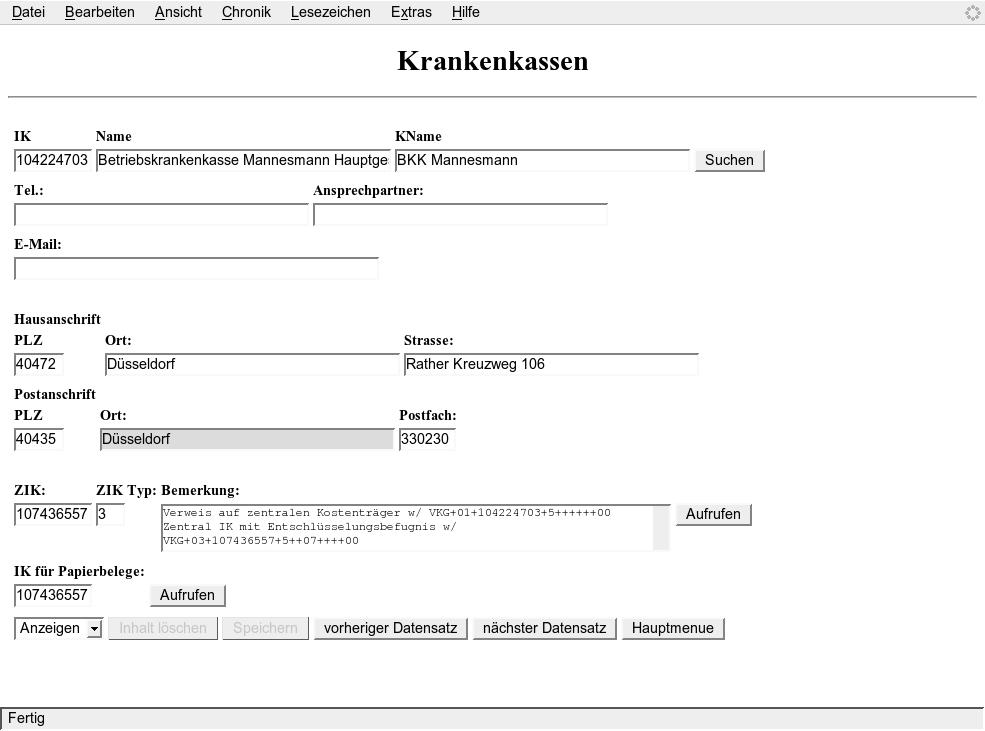
\includegraphics[width=9cm]{krankenkassen}
\caption{Krankenkassenerfassungsmaske\label{krankenkassenerfassung:fig}}
\end{figure}
\subsection{Beschreibung der Krankenkassenfelder}
Der Cursor steht nach Aufruf der Maske im Feld \feld{Name}, bzw. im ersten
leeren Feld nach der IK Nummer.
Folgende Felder sind auf der Maske vorhanden:
\begin{description}
\item[IK] 
Dieses Feld enthält die IK Nummer der Krankenkasse.
\item[Name]
Dieses Feld enthält den Namen der Krankenkasse. Hat die Krankenkasse einen
sehr langen Namen, ist nur der erste Teil des Names sichtbar.
Eine Prüfung ob der Nname erfasst wird, existiert an dieser Stelle nicht.
\item[KName] 
Das Feld enthält den Kurznamen der Krankenkasse. Dieser Name wird später
in der Rechnung angedruckt.
Eine Prüfung ob der Kurzname erfasst wird, existiert an dieser Stelle nicht.
\item[Tel.] 
Das Feld enthält die Telefonnummer der Krankenkasse, 
es können beliebige
Zeichen erfasst werden. Das Feld hat rein informativen Charakter 
und wird in der weiteren Anwendung
nicht mehr verwendet.
\item[E-Mail]
Das Feld enthält die E-Mail Adresse der Krankenkasse und ist i.d.R. nur 
für Datenannahmestellen gefüllt.
\end{description}

\paragraph{Hausanschrift}
\begin{description}
\item[PLZ] 
Das Feld enthält die PLZ zur Anschrift der Krankenkasse. 
Es wird in die 
spätere Rechnung übernommen. Es muss eine 5-stellige numerische Zahl
 erfasst werden. Das
bedeutet, eine 4-stellige PLZ, wie z.B. 04177 Leipzig,
muss mit führender Null erfasst werden. Ob
die PLZ im Sinne der Post wirklich gültig ist oder nicht, wird nicht
geprüft. Ein nicht korrekter Wert führt zu einer entsprechenden Fehlermeldung,
die durch Drücken des Knopfes \knopf{OK} bestätigt werden muss.
Das Speichern des Formulares mit ungültigen Werten ist nicht möglich.
Eine Prüfung, ob die PLZ erfasst wird, existiert an dieser Stelle nicht.
\item[Ort] 
Das Feld enthält den Ort zur Anschrift der Krankenkasse. Der Ort wird in die 
spätere Rechnung übernommen. Eine Prüfung, ob der Ort erfasst wird, exisiert
an dieser Stelle nicht.
\item[Strasse] 
Das Feld enthält die Strasse zur Anschrift der Krankenkasse, Die Strasse 
wird in die 
spätere Rechnung übernommen. Eine Prüfung, ob die Strasse erfasst wird, 
exisiert an dieser Stelle nicht.
\end{description}

\paragraph{Postanschrift}
Besitzt die Krankenkasse ein Postfach, sind die Felder unter der
Überschrift Postanschrift gefüllt. Da der Ort identisch ist, wird dieser aus
der Hausanschrift übernommen. Falls eine Postanschrift vorhanden ist,
wird die spätere Rechnung an die Postanschrift und nicht die Hausanschrift
verschickt.
\begin{description}
\item[PLZ] 
Das Feld enthält die PLZ zur Anschrift der Krankenkasse. 
Es wird in die 
spätere Rechnung übernommen. Es muss eine 5-stellige numerische Zahl
 erfasst werden. Das
bedeutet, eine 4-stellige PLZ, wie z.B. 04177 Leipzig,
muss mit führender Null erfasst werden. Ob
die PLZ im Sinne der Post wirklich gültig ist oder nicht, wird nicht
geprüft. Ein nicht korrekter Wert führt zu einer entsprechenden Fehlermeldung,
die durch Drücken des Knopfes \knopf{OK} bestätigt werden muss.
Das Speichern des Formulares mit ungültigen Werten ist nicht möglich.
Eine Prüfung, ob die PLZ erfasst wird, existiert an dieser Stelle nicht.
\item[Ort] 
Das Feld ist nich erfassbar und wird aus dem Feld \feld{Ort} der
Hausanschrift übernommen.
\item[Postfach] 
Das Feld enthält Nummer des Postfaches zur Anschrift der Krankenkasse.
Das Postfach wird in die 
spätere Rechnung übernommen. Eine Prüfung, ob ein Postfach erfasst wird, 
exisiert an dieser Stelle nicht.
\end{description}

\paragraph{}

\begin{description}
\item[ZIK]
\index{ZIK}
In diesem Feld ist eine IK Nummer angegeben, mit der die Krankenkasse
verknüpft ist. Dies kann z.B. ein Kostenträger oder einer Datenannahmestelle
sein.
\item[ZIK Typ]
\index{ZIK Typ}
In diesem Feld ist die Art der Verknüpfung zwischen Krankenkasse und der
``zentral IK'' angegeben. In \tinyHeb\/ existieren vier verschiedene Arten
von Verknüpfungen:

\begin{enumerate}
\item[0] 
Es existiert keine Verknüpfung.
\item[1]
Bei der im Feld \feld{ZIK} angegebenen IK Nummer handelt es sich um den
Kostenträger zur angezeigten Krankenkasse.
\item[2]
Bei der im Feld \feld{ZIK} angegebenen IK Nummer handelt es sich um eine
Datenannahmestelle ohne Entschlüsselungsbefugnis. Die angezeigte Krankenkasse
ist Datenannahmestelle mit Entschlüsselungsbefugnis. Die elektronische
Rechnung muss an die IK im \feld{ZIK} geschickt werden. Dabei handelt es
sich um den so genannten physikalischen Empfänger der Daten \cite{ktrdat}.
\item[3]
Bei der im Feld \feld{ZIK} angegebenen IK Nummer handelt es sich um eine
Datenannahmestelle mit Entschlüsselungsbefugnis.
\end{enumerate}

\item[Bemerkung]
In diesem Feld können beliebige Informationen zu Krankenkasse hinterlegt
werden. Im Rahmen des automatischen Einlesens der Kostenträgerdateien wird
dieses Feld überschrieben. Angzeigt werden Informationen aus den 
Kostenträgerdateien, die zur Ermittlung der Felder 
\feld{ZIK}, \feld{ZIK Typ} und \feld{IK für Papierbelege} genutzt wurden.
\item[IK für Papierbelege]
In diesem Feld ist die IK Nummer angegeben, an die die Papierbelege, bzw.
Urbelege geschickt werden müssen. Dieses Feld wird nur genutzt, wenn der
Parameter Belege auf 1 steht, siehe \vref{programmsteuerung_parm}.
\end{description}


\subsection{Beschreibung der Knöpfe im Krankenkassenmenue}
\begin{description}
\item[Suchen] 
Mit dem Knopf \knopf{Suchen} kann eine weitere Maske geöffnet
werden, über die Krankenkassen gesucht werden können. Die Beschreibung zu der
Suchmaske befindet sich in Abschnitt \vref{kassenauswahl:abs}.
\item[Aufrufen] 
Der Knopf \knopf{Aufrufen} hinter dem Feld
\feld{Bemerkung} wird nur angezeigt, wenn das Feld \feld{ZIK} gefüllt ist. 
Die im Feld \feld{ZIK} angezeigte IK Nummer wird in der Maske
Krankenkassen aufgerufen.
\item[Aufrufen] 
Der Knopf \knopf{Aufrufen} hinter dem Feld
\feld{IK für Papierbelege} wird nur angezeigt, 
wenn das Feld \feld{IK für Papierbelege} gefüllt ist. 
Die im Feld \feld{IK für Papierbelege} angezeigte IK Nummer wird in der Maske
Krankenkassen aufgerufen.
\item[Inhalt löschen] 
Der Knopf \knopf{Inhalt löschen} ist nur dann
Aktiv, wenn in dem
Pop Down Menue vor dem Knopf der Wert Neu ausgewählt wurde. Wird der Knopf
gedrückt, werden die Feldinhalte aller Felder der Maske gelöscht und das
Pop Down Menue springt auf den Wert Anzeigen. Der Datensatz selbst wird
nicht gelöscht.
\item[Speichern/ Löschen] Der Knopf \knopf{Speichern} ist nur dann aktiv,
wenn im
Auswahlmenue entweder der Wert Neu oder Ändern gewählt wird. 
\par
Falls \knopf{Neu}
ausgewählt wurde, wird eine neue Krankenkasse in der Datenbank gespeichert
und das Pop Down Menue springt auf den Wert Anzeigen. Neben den oben
beschriebenen Plausibilitäten Prüfungen findet beim Speichern keine weitere
Prüfung statt.\par
Falls \knopf{Ändern} gewählt wurde, wird der Datensatz, der sich in der Datenbank
befindet mit den angezeigten Werten überschrieben und das Pop Down Menue
springt auf den Wert Anzeigen. Neben den oben beschriebenen
Plausibilitätenprüfungen finden keine weiteren Prüfungen statt.

Falls im Pop Down Menue \knopf{Löschen} ausgewählt wurde, erhält der Knopf die
Beschriftung Löschen. Durch Drücken des Knopfes wird die Krankenkasse aus der
Datenbank gelöscht. Alle Feldinhalte der Felder der Maske werdem gelöscht 
und das Auswahlmenue
steht auf den Wert Anzeigen. 
\item[vorheriger Datensatz] 
Dieser Knopf ist nur dann aktiv, wenn der Wert
des Pop Down Menues auf Anzeigen steht. Durch Drücken des Knopfes wird auf
den vorherigen Datensatz in der Datenbank gesprungen. Der vorherige Datensatz
ist derjenige, mit der nächst kleineren IK Nummer, als die im Feld 
\feld{IK} angezeigte. Ist
man am ersten Datensatz angekommen, bleibt dieser in der Maske erhalten.
\item[nächster Datensatz] 
Dieser Knopf ist nur dann aktiv, wenn der Wert
des Pop Down Menues auf Anzeigen steht. Durch Drücken des Knopfes wird auf
den nächsten Datensatz in der Datenbank gesprungen. Der nächste Datensatz
ist derjenige, mit der nächst höheren IK Nummer, als die im Feld 
\feld{IK} aktuell angezeigte. Ist
man am letzten Datensatz angekommen, bleibt dieser in der Maske erhalten.
\item[Hauptmenue] 
Über diesen Knopf gelangt man in die Maske Hauptmenue.
Dabei ist zu beachten, dass nicht überprüft wird, ob Änderungen oder Neu
erfasste Daten gespeichert wurden. Es wird sofort in die Maske Hauptmenue
gesprungen.
\end{description}

Sind alle Felder erfasst, können die Daten gespeichert werden. Dazu ist
es notwendig im Pop Down Menue unten links den Wert 'Neu' auszuwählen.
Sobald dies geschehen ist, wird der Knopf \knopf{Speichern} aktiv 
geschaltet. Drückt man jetzt den Knopf \knopf{Speichern} werden die Daten
zur Krankenkasse permanent abgelegt. Nach dem Speichern wird die Auswahl im 
Pop Down Menue unten links auf den Wert 'Anzeigen' gesetzt.




\section{Kassenauswahl}\label{kassenauswahl:abs}
In diesem Absatz ist beschrieben, wie Krankenkassen im Datenbestand gesucht und
ausgewählt werden können.
In der Regel erfolgt der  Aufruf der Maske aus der 
Krankenkassenerfassungsmaske (siehe
Seite \pageref{krankenkassenerfassung:fig}) 
über den Knopf \knopf{Suchen}. Einen analogen Knopf findet man in der Maske 
Stammdatenerfassung (siehe Seite \pageref{stammdatenerfassung:fig}).
Klickt man auf den Knopf \knopf{Suchen} wird ein neues Fenster mit der
Überschrift ``Krankenkasse suchen'' geöffnet\footnote{sollte das Fenster noch geöffnet sein, wird es in den Vordergrund des Bildschirms geholt.}

(Abbildung \vref{kassenauswahl:fig}). Über die Felder \feld{IK,
Name, KName, Ort, PLZ Hausanschrift, PLZ Postfach} ist es möglich die
Suchkriterien vorzugeben, d.h. es werden bei der Suche nur die Krankenkassen
ausgegeben, bei denen alle vorgegebenen Werte vorhanden sind. Dabei ist
folgendes für die Felder zu beachten:

\begin{figure}[h]
\centering
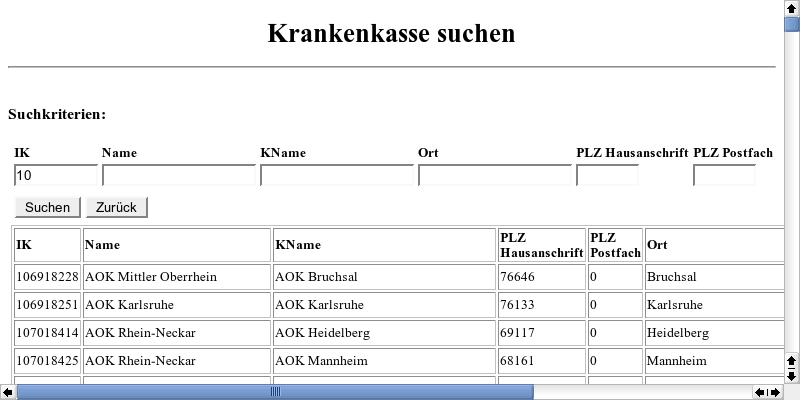
\includegraphics[width=9cm]{kassenauswahl}
\caption{Kassenauswahlmaske\label{kassenauswahl:fig}}
\end{figure}

\begin{description}
\item[IK] Es wird nur nach den Krankenkassen gesucht, bei denen die IK Nummer 
einen Teil des Feldes enthält.
Wird z.B. im Feld \feld{IK} ``70184'' erfasst,
würde IK 107018414, 107018425 und 107018436 ermittelt werden.
\item[Name] Es wird nur nach den Krankenkassen gesucht, bei denen der
Name einen Teil des Feldes enthält
Wird z.B. im Feld \feld{Name} ``Solingen'' erfasst,
würden alle Krankenkassen deren Name ``Solingen'' enthält ermittelt werden.
Wird z.B. im Feld \feld{Name} ``Solingen'' erfasst, würde
``AOK Solingen'', ``Betriebskrankenkasse Mannesmann Geschäftsstelle Solingen''
und ``IKK Nordrhein RD Solingen'' ermittelt werden.
\item[KName]
Es wird nur nach den Krankenkassen gesucht, bei denen der
Name einen Teil des Feldes enthält
Wird z.B. im Feld \feld{KName} ``IKK Nordrhein'' erfasst,
werden alle Krankenkassen ermittelt, deren Name ``IKK Nordrhein'' enthält.
\item[Ort] 
Es wird nur nach den Krankenkassen gesucht, bei denen der Ort einen Teil
des Feldes enthält.
Wird z.B. im Feld \feld{Ort} ``Fürth'' erfasst, werden
die Krankenkassen in ``Fürth'' und ``Wipperfürth'' ermittelt.
\item[PLZ Hausanschrift] 
Es wird nur nach den Krankenkassen gesucht, bei denen die Postleitzahl der
Hausanschrift mit denen im Feld angegebenen Werten beginnt.
Wird z.B. im Feld \feld{PLZ Hausanschrift} ``4271'' erfasst, werden die
Krankenkassen ``Betriebskrankenkasse Bergisch Land Die Bergische Krankenkasse'' und ``Betriebskrankenkasse Krups/Zwilling'' ermittelt.
\item[PLZ Postfach] 
Es wird nur nach den Krankenkassen gesucht, bei denen die Postleitzahl des
Postfaches mit denen im Feld angegebenen Werten beginnt.
Wird z.B. im Feld \feld{PLZ Hausanschrift} ``427'' erfasst, werden die
Krankenkassen ``Betriebskrankenkasse Bergisch Land Die Bergische Krankenkasse'', ``Betriebskrankenkasse Krups/Zwilling'' und 
``IKK Nordrhein RD für den Kreis Mettmann'' ermittelt.
\end{description}
Die Suche Startet, nachdem der Knopf \knopf{Suchen} gedrückt wird.
Das Ergebnis der Suche wird unmittelbar unter den Suchkriterien ausgegeben.

Über den Knopf \knopf{Auswählen} werden die Daten der Krankenkasse in die Maske
übernommen, aus der die Suchfunktion aufgerufen wurde. 
Die Maske ``Krankenkasse suchen''
wird danach geschlossen.

Falls keine Krankenkasse den gewünschten Suchkriterien entspricht, 
kann entweder durch Klicken des Knopfes \knopf{Zurück} die 
Maske ``Krankenkasse suchen''
geschlossen, oder es können andere Suchkriterien erfasst werden.



\section{Erfassen von Rechnungsposten\label{rechnungspostenerfassung:kap}}
\index{Rechnungsposten}
In diesem Abschnitt werden die Möglichkeiten der Rechnungspostenerfassung
aufgezeigt. Es wird beschrieben, welche Positionsnummern automatisch
angewählt werden, welche Plausibilitätenprüfungen existieren, 
aber auch wo die Grenzen von \tinyHeb\/ sind. Es
ist insbesondere zu beachten, dass \tinyHeb\/ der Hebamme nicht das
Denken abnimmt ;-), sondern eine Hilfe für die Abrechnung gegenüber den
Krankenkassen, bzw. den privaten Kundinnen darstellt.

Es gibt verschiedene Wege um in die Rechnungsposten Erfassung zu gelangen.
Aus dem Hauptmenue (Abbildung \vref{einstieg:fig})
gelangt man über den Link \verb|Rechnungsposten erfassen|
in die Maske zur Rechnungspostenerfassung (Abbildung 
\vref{rechnungspostenerfassen:fig}). Aus der Maske Rechnungsgenerierung
über den Knopf \knopf{Rechnungsposten erfassen} und aus der Maske Stammdaten
über den Knopf \knopf{Rechnungsposten erfassen}. Erfolgt der Aufruf
aus den Masken Rechnungsgenerierung oder Stammdaten, werden die Daten
der aktuell in der Anzeige befindlichen Frau in die Maske Rechnungsposten
erfassen übernommen. 

\begin{figure}[ht]
\centering
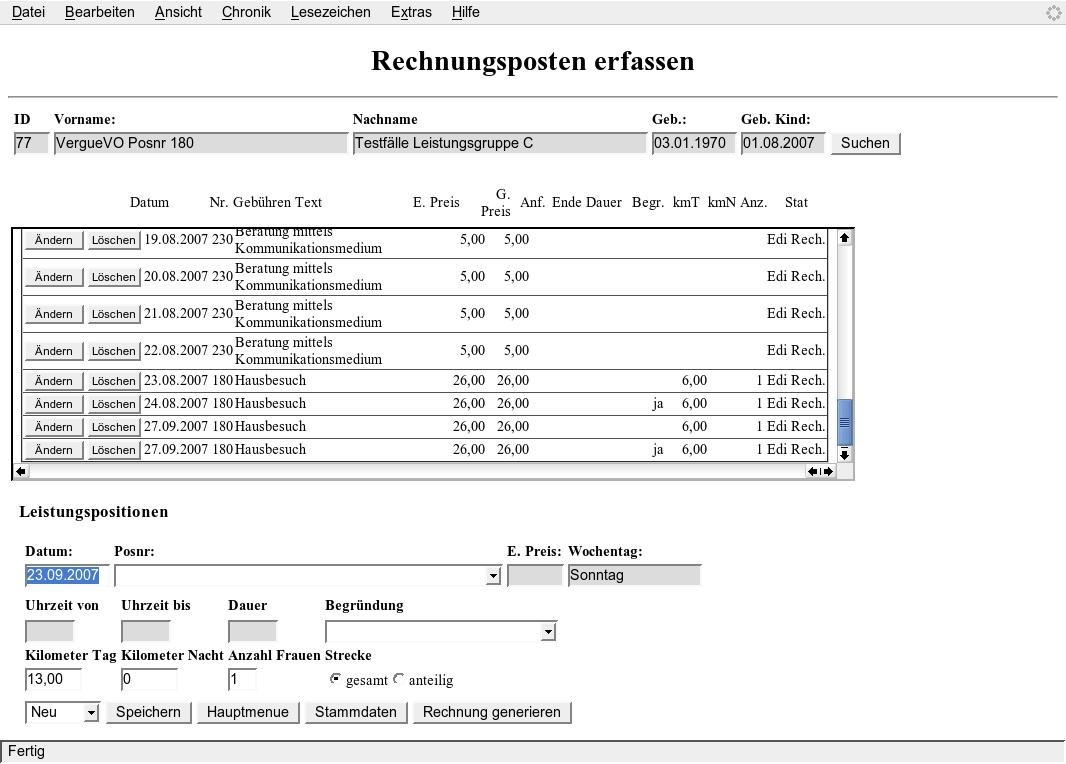
\includegraphics[width=9cm]{rechnungspostenerfassen}
\caption{Rechnungsposten erfassen\label{rechnungspostenerfassen:fig}}
\end{figure}

Wie schon in der Kurzanleitung beschrieben, ist
die Maske in drei Teile gegliedert. Im oberen Teil werden Daten zur Frau
angezeigt, die aktuell bearbeitet wird. In der Mitte werden die bisher
erfassten Rechnungsposten angzeigt. Im unteren Teil findet die Erfassung
der einzelnen Rechnungsposten statt.

\paragraph{Daten zur Frau}
Im oberen Bereich werden die wesentlichen Daten zur Frau angezeigt. Dazu
gehören, die ID, Vor- und Nachname, sowie das Geburtsdatum der Frau und
des Kindes. Diese Felder können nicht erfasst werden. Soll eine andere
Frau ausgewählt werden, muss dies über den Knopf \knopf{Suchen} geschehen.
Die Beschreibung zur Suchmaske befindet sich im Abschnitt 
\vref{frauenauswahl:abs}. Es werden keine Informationen in die Suchmaske
übernommen.

\paragraph{bisher erfasste Rechnungsposten}
Im mittleren Abschnitt werden die bisher erfassten Posten angezeigt.
Es werden die Felder Datum (Datum der Leistungserbringung), die 
Positionsnummer, die Kurzbezeichnung der Positionsnummer, der Preis
der einzelnen Positionsnummer, der Gesamtpreis, ggf. Anfang und Ende
sowie die Dauer des Leistungszeitraumes, ob eine Begründung erfasst wurde,
die Kilometeranzahl Tag (kmT) und Nacht (kmN), wie viele Frauen besucht
wurden und der Status der Rechnungsposition gezeigt.

Der Gesamtpreis ist in der Regel identisch mit dem Einzelpreis. Bei
Positionsnummern, die nach Dauer berechnet werden, wie z.B.
``Hilfe bei Beschwerden'', wird je nach Dauer und Positionsnummer die Dauer
mit dem Einzelpreis multipliziert und angezeigt.
Genau in diesen Fällen wird angezeigt, wann mit der Leistung begonnen, bzw.
wann sie beendet wurde. 

Ist bei einem Rechnungsposten nur die Anfangszeit erfasst worden\footnote{dies
ist sinnvoll, damit die entsprechenden
Positionsnummern für Nacht, Sonn- und Feiertagszuschlag automatisch ermittelt 
werden können}, z.B.
bei Positionsnummer 180 ``Hausbesuch nach der Geburt'' wird nur die 
Anfangszeit angezeigt, Ende und Dauer bleiben leer.
In allen anderen Fällen bleiben die Felder für
Anfang, Ende und Dauer leer. 
Bei Anzeige des Einzel- und Gesamtpreises wird die HebGV zu Grunde gelegt.
Falls es sich um eine Privatpatientin\index{Privatpatientin}
 handelt, werden die einzelnen
Rechnungsposten mit dem korrekten Preis erst in der Maske 
Rechnungsgenerierung angezeigt.

Ist eine Begründung bei der einzelnen Position erfasst worden, wird unter
Begr. ``ja'' angezeigt, auch dieses Feld wird nur angezeigt, wenn eine
Begründung erfasst wurde.

Analoges gilt für die Felder kmT und kmN, sowie Anzahl. Diese Felder werden
nur angezeigt, wenn Kilometer erfasst wurden.

Ganz Rechts wird der Status der einzelnen Position angezeigt, folgende
Status sind möglich.
\begin{description}
\item[in bearb.] 
Für diesen Posten wurde noch keine Rechnung erstellt.
\item[Rechnung] 
Für diesen Posten wurde eine Papierrechnung erstellt. 
\item[Edi Rech.] 
Für diesen Posten wurde eine elektronische Rechnung erstellt. 
\item[Mahnung]
Für diesen Posten wurde bereits eine Mahnung erstellt, dabei wird angegeben, 
wie viele Mahnung bisher erstellt wurden.
\item[erl.] 
Dieser Rechnungsposten wurde schon beglichen.
\end{description}

Ist der Status ungleich ``in bearb.'', ist eine Änderung oder Löschung
dieses Postens nicht mehr möglich.
Über den Knopf \knopf{Ändern} werden die Informationen der entsprechenden
Position in den unteren Bereich der Maske übernommen und die Daten können
geändert werden.
Über den Knopf \knopf{Löschen} wird die entsprechende Position sofort
gelöscht. Gibt es von dieser Position abhängige Positionsnummern, werden
diese ebenfalls gelöscht. D.h. wenn z.B. ein Rechnungsposten für 
Positionsnummer 190 ``Zuschlag 1. Besuch nach der Geburt'' gelöscht wird,
wird die entsprechende Materialpauschale ebenfalls gelöscht. Aber bitte
keine Sorgen machen, \tinyHeb\/ ermittelt automatisch, ob für einen
anderen Tag der ``Zuschlag 1. Besuch nach der Geburt'' berechnet werden
muss und wird dann auch die entsprechende Materialpauschale automatisch
auswählen.

\subsection{Erfassung der Rechnungspositionen}
In diesem Abschnitt werden zunächst die einzelnen Felder und Knöpfe
beschrieben. Danach schließt sich eine Beschreibung für jede
Positionsnummer aus der Hebammen-Vergütungs\-ver\-ordnung, bzw. HebGV an, 
mit einer Beschreibung, welche
Plausibilitätenprüfungen für die jeweilige Positionsnummer existieren,
respektive, welche weiteren Positionsnummern automatisch angewählt werden.

\subsection{Felder und Knöpfe}
Folgende Felder sind in der Maske vorhanden:

\begin{description}
\item[Datum] 
Datum der Leistungserbringung. In diesem Feld ist zu erfassen, wann
die Leistung erbracht wurde, bzw. an welchem Tag eine Auslage entstanden ist.
D.h. wann z.B. eine Salbe verabreicht wurde.
Die Erfassung muss im Format TT.MM.JJJJ oder TT.MM.JJ erfolgen. 
Wird das Datum im Format TT.MM.JJ erfasst, erfolgt nach Verlassen des
Feldes automatisch die Ermittlung und Darstellung der 4-stelligen Jahreszahl.
Ein ungültiges Datum führt zu der Fehlermeldung: Bitte gültiges Datum erfassen.
Das Speichern des Formulares mit ungültigen Werten ist nicht möglich.
\item[Posnr]
Über dieses Pop-Down-Feld kann die entsprechende Positionsnummer zu der
erbrachten Leistung ausgewählt werden, bzw. die interne Positionsnummer
für die entsprechende Materialien.
\item[Anzahl Kurse]
Dieses Feld wird nur dann auf der Maske dargestellt, wenn Positionsnummer 7,
070, 40 oder Positionsnummer 270 ausgewählt wird. 
In diesen Fällen lässt sich erfassen,
wie viele Kurse durchgeführt wurden. Die jeweiligen einzelnen
Rechnungsposten werden automatisch generiert. Dazu werden die Werte aus
den Feldern \feld{Uhrzeit von} und \feld{Uhrzeit bis} übernommen, 
der Inhalt des Feldes \feld{Datum} wird jeweils um sieben Tage erhöht.
\item[E. Preis] 
Dieses Feld enthält den Einzelpreis zu der im Feld \feld{Posnr} ausgewählten
Positionsnummer, es wird angezeigt, sobald das Feld Positionsnummer
verlassen wurde. Das Feld ist nicht erfassbar. Es wird immer der
Preis gemäß HebGV angezeigt. Falls es sich um eine Privatkundin handelt,
wird erst in der Maske Rechnungsgenerierung der korrekte Preis angezeigt.
\item[Wochentag]
Dieses Feld enthält den Wochentag zu dem im Feld \feld{Datum} erfassten Datum.
Es wird aktualisiert, sobald das Feld \feld{Datum} verlassen wird.
Das Feld ist nicht erfassbar.
\item[Uhrzeit von]
Dieses Feld enthält die Uhrzeit ab der mit der Leistungserbringung begonnen
wurde. Es ist für alle Positionsnummern erfassbar. Zwingend ist es zu erfassen,
wenn es sich um eine Positionsnummer handelt,
bei der eine Zeitangabe notwendig ist, das ist z.B. bei Positionsnummer 050
``Hilfe bei Beschwerden'' der Fall. Bei allen Positionsummern für die ein
Zuschlag erfolgen kann und diese nach Beginn der Leistung berechnet wird, 
z.B. Positionsnummer 180. 
Das Feld muss im Format HH:MM oder
HHMM erfasst werden. Eine ungültige Uhrzeit führt zu der Fehlermeldung:
Bitte gültige Uhrzeit im Format hh:mm erfassen. Das Speichern des Formulares
mit ungültigen Werten ist nicht möglich.

\item[Uhrzeit bis]
Die Beschreibung ist analog dem Feld \feld{Uhrzeit von}. Es muss der
Zeitpunkt erfasst werden, bis zu dem die Leistung erbracht wurde.
Wichtig ist die Erfassung bei Positionsnummern, bei denen Zuschläge nach dem
Ende der Leistungserbringung berechnet werden, z.B. Positionsnummer 160.
\item[Dauer]
Das Feld Dauer lässt sich nicht erfassen und hat in der aktuellen Version
noch keine Funktionalität. In einer späteren Version soll hier nach erfassen
der Felder \feld{Uhrzeit von} und \feld{Uhrzeit bis} sofort die entsprechende
Dauer angzeigt werden.
\item[Begründung]
Über dieses Pop-Down-Feld kann eine Begründung ausgewählt werden. Sind
die angegebenen Begründungen nicht ausreichend, können über die
Programmsteuerungsparameter neue hinzugefügt werden. Wie dies geht ist 
in Abschnitt \vref{programmsteuerungsparameter} beschrieben. 
Eine Begründung ist \textbf{immer} zu erfassen,
wenn mit diesem Posten ein Beleg verbunden ist, wie z.B. ein 
ärztliches Attest. Dann ist die Begründung ``Attest (auf ärztliche
Anordnung)'' auszuwählen. Auf diese Begründung legen verschieden 
Datenannahmestellen ausdrücklich wert. Wird als Begründung ``Attest
(auf ärztliche Anordnung)'' ausgewählt, werden zwei neue Felder
\feld{Schlüssel} und {Text} zur Erfassung von Diagnose Angaben 
eingeblendet.
\item[Schlüssel]
Dieses Feld wird nur auf der Maske dargestellt, wenn als Begründung
``Attest (auf ärztliche Anordnung)'' im Feld \feld{Begründung}
ausgewählt wurde. In diesem Fall lässt sich der Diagnoseschlüssel
\index{Diagnoseschlüssel} aus der entsprechenden Anordnung
in diesem Feld erfassen.
\item[Text]
Dieses Feld wird nur auf der Maske dargestellt, wenn als Begründung
``Attest (auf ärztliche Anordnung)'' im Feld \feld{Begründung}
ausgewählt wurde. In diesem Fall lässt sich der Diagnosetext
\index{Diagnosetext} aus der entsprechenden Anordnung
in diesem Feld erfassen.
\item[Kilometer Tag]
\index{Wegegeld}
In diesem Feld kann die Anzahl der bei Tag zurückgelegten Kilometer für die
entsprechende Positionsnummer erfasst werden. Es können nur numerische
Werte erfasst werden. Das Feld ist nur dann zur Erfassung freigeschaltet,
wenn für die entsprechende Positionsnummer Wegegeld abgerechnet werden
kann. D.h. für Positionsnummer 190 ``Zuschlag für den ersten Besuch nach
der Geburt'' ist das Feld für die Erfassung gesperrt\footnote{durch
Änderung der Leistungsartenparameter wie in  Abschnitt
\vref{leistungsarten:abs} beschrieben, kann dies individuell angepasst
werden}.
\item[Kilometer Nacht]
In diesem Feld kann die Anzahl der bei Nacht zurückgelegten Kilometer für die
entsprechende Positionsnummer erfasst werden. Es können nur numerische
Werte erfasst werden. Das Feld ist nur dann zur Erfassung freigeschaltet,
wenn für die entsprechende Positionsnummer Wegegeld abgerechnet werden
kann. D.h. für Positionsnummer 190 ``Zuschlag für den ersten Besuch nach
der Geburt'' ist das Feld für die Erfassung gesperrt.
\item[Anzahl Frauen]
In diesem Feld kann erfasst werden, wieviele Frauen im Rahmen der 
zurückgelegten Kilometer Anzahl besucht wurden. Wird in diesem Feld nichts
erfasst, geht \tinyHeb\/ davon aus, dass eine Frau besucht wurde.
\item[Strecke]
Über dieses Feld kann gesteuert werden, ob es sich bei der zurückgelegten
Strecke um die gesamte oder die anteilige Wegstrecke handelt. D.h.
es gibt zwei Möglichkeiten, wie die Wegstrecke erfasst werden kann.
Wurden z.B. drei Frauen besucht und insgesamt 24 Kilometer am Tag
zurückgelegt, kann dies wie folgt erfasst werden:

\begin{enumerate}
\item 24 im Feld \feld{Kilometer Tag}, 3 bei \feld{Anzahl Frauen},
bei Strecke \feld{gesamt} anklicken.
\item 8 im Feld \feld{Kilometer Tag}, 3 bei \feld{Anzahl Frauen},
bei Strecke \feld{anteilig} anklicken.
\end{enumerate}
\end{description}

\paragraph{Folgende Knöpfe sind im unteren Teil der Maske vorhanden:}

\begin{description}
\item[Neu]
Wird in dem Pop Down Feld links der Wert Neu ausgewählt, kann über
den Knopf \knopf{Speichern} die erfasste Leistungsposition gespeichert
werden.
\item[Ändern]
Wird in dem Pop Down Feld links der Wert Ändern ausgewählt, kann
über den Knopf \knopf{Speichern} die angezeigte Leistungsposition 
geändert werden. Bei der Änderung werden abhängige Positionsnummern
automatisch mit geändert. D.h., wird z.B. der erste Hausbesuch nach
der Geburt geändert, wird überprüft, ob es sich noch immer um den
ersten Hausbesuch handelt\footnote{dies kann sich durch die Eingabe 
eines neuen Datums 
ändern.}, falls dies nicht der Fall ist, wird automatisch der erste
Hausbesuch gesucht und auch die entsprechende Materialpauschale 
angepasst. Ist die Änderung der Daten nicht möglich, wird eine
Fehlermeldung ausgegeben.
\item[Hauptmenue] 
Über diesen Knopf gelangt man in die Maske Hauptmenue.
Dabei ist zu beachten, dass nicht überprüft wird, ob Änderungen oder Neu
erfasste Daten gespeichert wurden. Es wird sofort in die Maske Hauptmenue
gesprungen.
\item[Stammdaten]
Über diesen Knopf gelangt man in die Stammdatenmaske.
Die ``in Bearbeitung befindlichen Frau'' wird automatisch in der
Stammdatenmaske  aufgerufen.
\item[Rechnung generieren]
Über diesen Knopf gelangt man in die Maske zur Rechnungsgenerierung.
Die Daten der ``in Bearbeitung befindliche Frau'' wird automatisch in der 
Maske Rechnungsgenerierung aufgerufen.
\end{description}



\subsection{die einzelnen Positionsnummern der Hebammen-Vergütungsvereinbarung}
\index{Hebammen-Vergütungsvereinbarung}
\index{Positionsnummern}
In der folgenden Tabelle sind alle Positionsnummern der 
Hebammen-Vergütungsvereinbarung
aufgeführt, sowie die in \tinyHeb\/ implementierten Plausibilitätenprüfungen.
Es ist zu beachten, dass in der Vergütungsvereinbarung ggf. Einschränkungen 
gemacht werden,
die in der aktuellen Version von \tinyHeb\/ nicht geprüft werden.
Wenn möglich habe ich dies in einer Fußnote kenntlich gemacht.
D.h. es werden nur die angegebenen Plausibilitätenprüfungen durchgührt und
auch nur die Positionsnummern automatisch angewählt, die angegeben sind.
Veränderungen an den Leistungsartenparametern wie in Abschnitt
\vref{leistungsarten:abs} beschrieben, führen selbstverständlich zu 
anderen als den hier angebenen Prüfungen.


\bottomcaption{Positions\-nummern der Hebammen-Vergütungs\-vereinbarung}
\tablehead
{\hline \bfseries Positions\-nummer&\bfseries Beschreibung\\ \hline}

\tabletail
{\hline \multicolumn{2}{r}{\emph{Fortsetzung auf der nächsten Seite}}\\}

\tablelasttail{\hline}
\begin{mpsupertabular}{|>{\centering}p{1.9cm}|p{11.6cm}|}
010&
\textbf{Beratung der Schwangeren, auch mittels Kommunikationsmedium}
\paragraph{Plausiprüfungen}
\begin{enumerate}
\item
Die Erfassung ist nur zulässig, wenn das Feld \feld{Datum} kleiner 
oder gleich dem Geburtsdatum des Kindes ist. Ist das Geburtsdatum des
Kindes nicht bekannt, wird diese Prüfung nicht durchgeführt.
\item
Die Positionsnummer darf maximal 12 mal erfasst werden.
\item
Die Positionsnummer darf nicht mit den Positionsnummern 020, 030, 040, 050,
051, 060 und 080 am
selben Tag erfasst werden.
\item 
Bei mehrmaliger Erbringung der Leistung ist dies mit Angabe der jeweiligen
Uhrzeit zu begründen.
\end{enumerate}
\paragraph{automatisch gewählte Positionsnummern}
keine.
\\ \hline


020&
\textbf{Vorgespräch über Fragen der Schwangerschaft und Geburt}
\paragraph{Plausiprüfungen}
\begin{enumerate}
\item
Die Erfassung ist nur zulässig, wenn das Feld \feld{Datum} kleiner 
oder gleich dem Geburtsdatum des Kindes ist. Ist das Geburtsdatum des
Kindes nicht bekannt, wird diese Prüfung nicht durchgeführt.
\item
Die Felder \feld{Uhrzeit von} und \feld{Uhrzeit bis} müssen erfasst 
sein.
\item
Die Beratungsdauer muss mindestens 30 Minuten betragen.
\item
Die Beratungsdauer darf 60 Minuten nur dann überschreiten, wenn als
Begründung ``geplante Hausgeburt'' erfasst wurde.
\item
Die Beratungsdauer darf 90 Minuten nicht überschreiten.
\item
Die Positionsnummer kann nur mit Begründung ``geplante Hausgeburt'' mehr als
einmal erfasst werden.
\item
Die Positionsnummer kann maximal 2 mal erfasst werden.
\item
Es wird geprüft, ob für die angegebene Uhrzeit in dieser Positionsnummer
schon ein Rechnungsposten erfasst ist. Auch überschneidene Uhrzeiten
werden geprüft, z.B. führen 10:00 bis 12:00 und 11:00 bis 13:00 zu einer
Fehlermeldung.
\item
Die Positionsnummer darf nicht mit den Positionsnummern 010, 030, 040, 050,
051, 060 und 080 am selben Tag erfasst werden.
\end{enumerate}
\paragraph{automatisch gewählte Positionsnummern}
keine
\\ \hline



030&
\textbf{Vorsorgeuntersuchung der Schwangeren}
\paragraph{Plausiprüfungen}
\begin{enumerate}
\item
Die Erfassung ist nur zulässig, wenn das Feld \feld{Datum} kleiner 
oder gleich dem Geburtsdatum des Kindes ist. Ist das Geburtsdatum des
Kindes nicht bekannt, wird diese Prüfung nicht durchgeführt.
\item
Die Positionsnummer darf nicht mit den Positionsnummern 010, 020 am
selben Tag erfasst werden.
\end{enumerate}
\paragraph{automatisch gewählte Positionsnummern}
\begin{enumerate}
\item
Es wird zusätzlich automatisch Positionsnummer 340 (Pauschale für
Vorsorgeuntersuchung ausgewählt).
\end{enumerate}
\\ \hline

040&
\textbf{Entnahme von Körpermaterial}
\paragraph{Plausiprüfungen}
\begin{enumerate}
\item
Die Erfassung ist nur zulässig, wenn das Feld \feld{Datum} kleiner 
oder gleich dem Geburtsdatum des Kindes ist. Ist das Geburtsdatum des
Kindes nicht bekannt, wird diese Prüfung nicht durchgeführt.
\item
Die Positionsnummer darf nicht mit den Positionsnummern 010, 020 am
selben Tag erfasst werden.
\end{enumerate}
\paragraph{automatisch gewählte Positionsnummern}
\begin{enumerate}
\item
keine
\end{enumerate}
\\ \hline


050&
\textbf{Hilfe bei Beschwerden}
\paragraph{Plausiprüfungen}
\begin{enumerate}
\item
Die Erfassung ist nur zulässig, wenn das Feld \feld{Datum} kleiner 
oder gleich dem Geburtsdatum des Kindes ist. Ist das Geburtsdatum des
Kindes nicht bekannt, wird diese Prüfung nicht durchgeführt.
\item
Die Felder \feld{Uhrzeit von} und \feld{Uhrzeit bis} müssen erfasst sein.
\item
Es wird geprüft, ob für die angegebene Uhrzeit in dieser Positionsnummer
schon ein Rechnungsposten erfasst ist. Auch überschneidene Uhrzeiten
werden geprüft, z.B. führen 10:00 bis 12:00 und 11:00 bis 13:00 zu einer
Fehlermeldung.
\item
Die Positionsnummer darf nicht mit den Positionsnummern 010, 020 am
selben Tag erfasst werden.
\item
Dauert die Leistung länger als 3 Stunden, so ist eine Begründung anzugeben.
\end{enumerate}
\paragraph{automatisch gewählte Positionsnummern}
\begin{enumerate}
\item
Nachts, an Samstagen nach 12:00, Sonn- und Feiertagen wird automatisch 
Positions\-nummer 051 ausgewählt.
\end{enumerate}
\\ \hline


051&
\textbf{Hilfe bei Beschwerden Sa, So, Nacht}
\paragraph{Plausiprüfungen}
\begin{enumerate}
\item
Die Erfassung ist nur zulässig, wenn das Feld \feld{Datum} kleiner 
oder gleich dem Geburtsdatum des Kindes ist. Ist das Geburtsdatum des
Kindes nicht bekannt, wird diese Prüfung nicht durchgeführt.
\item
Die Felder \feld{Uhrzeit von} und \feld{Uhrzeit bis} müssen erfasst sein.
\item
Es wird geprüft, ob für die angegebene Uhrzeit in dieser Positionsnummer
schon ein Rechnungsposten erfasst ist. Auch überschneidene Uhrzeiten
werden geprüft, z.B. führen 10:00 bis 12:00 und 11:00 bis 13:00 zu einer
Fehlermeldung.
\item
Die Positionsnummer darf nicht mit den Positionsnummern 010, 020 am
selben Tag erfasst werden.
\item
Dauert die Leistung länger als 3 Stunden, so ist eine Begründung anzugeben.
\item
Die Erfassung ist nur zulässig Nachts, an Samstagen nach 12:00, 
Sonn- und Feiertagen.
\end{enumerate}
\paragraph{automatisch gewählte Positionsnummern}
keine.
\\ \hline


060&
\textbf{CTG Überwachung}
\paragraph{Plausiprüfungen}
\begin{enumerate}
\item
Die Erfassung ist nur zulässig, wenn das Feld \feld{Datum} kleiner 
oder gleich dem Geburtsdatum des Kindes ist. Ist das Geburtsdatum des
Kindes nicht bekannt, wird diese Prüfung nicht durchgeführt.
\item
Die Positionsnummer darf nicht mit den Positionsnummern 010, 020 am
selben Tag erfasst werden.
\item
Es wird geprüft, ob als Begründung ``Attest (auf ärztliche Anordnung)'' 
erfasst wurde, wenn diese Positionsnummer mehr als zweimal an
einem Tag erfasst wird.
\end{enumerate}
\paragraph{automatisch gewählte Positionsnummern}
keine.
\\ \hline


070&
\textbf{Geburtsvorbereitung in der Gruppe}
\paragraph{Plausiprüfungen}
\begin{enumerate}
\item
Die Erfassung ist nur zulässig, wenn das Feld \feld{Datum} kleiner 
oder gleich dem Geburtsdatum des Kindes ist. 
Für den Fall, dass über das Feld \feld{Anzahl Kurse} ``zu viele``
Kurse ausgewählt wurden, wird nur die maximal mögliche Anzahl von Kursen
gespeichert. 

Ist das Geburtsdatum des
Kindes nicht bekannt, wird diese Prüfung nicht durchgeführt.
\item
Die Felder \feld{Uhrzeit von} und \feld{Uhrzeit bis} müssen erfasst sein.
\item
Es wird geprüft, ob für die angegebene Uhrzeit in dieser Positionsnummer
schon ein Rechnungsposten erfasst ist. Auch überschneidene Uhrzeiten
werden geprüft, z.B. führen 10:00 bis 12:00 und 11:00 bis 13:00 zu einer
Fehlermeldung.
\item
Es wird geprüft, ob ob die Summe aller bisher erfassten Stunden größer
ist als 14 Stunden. Ist dies der Fall, kann die Position nicht gespeichert
werden. Für den Fall, dass über das Feld \feld{Anzahl Kurse} ``zu viele``
Kurse ausgewählt wurden, wird nur die maximal mögliche Anzahl von Kursen
gespeichert.
\end{enumerate}
\paragraph{automatisch gewählte Positionsnummern}
keine
\\ \hline


080&
\textbf{Geburtsvorbereitung bei Einzelunterweisung}
\paragraph{Plausiprüfungen}
\begin{enumerate}
\item
Die Erfassung ist nur zulässig, wenn das Feld \feld{Datum} kleiner 
oder gleich dem Geburtsdatum des Kindes ist. Ist das Geburtsdatum des
Kindes nicht bekannt, wird diese Prüfung nicht durchgeführt.
\item
Die Positionsnummer darf nicht mit den Positionsnummern 010, 020 am
selben Tag erfasst werden.
\item
Die Felder \feld{Uhrzeit von} und \feld{Uhrzeit bis} müssen erfasst sein.
\item
Es wird geprüft, ob für die angegebene Uhrzeit in dieser Positionsnummer
schon ein Rechnungsposten erfasst ist. Auch überschneidene Uhrzeiten
werden geprüft, z.B. führen 10:00 bis 12:00 und 11:00 bis 13:00 zu einer
Fehlermeldung.
\item
Es wird geprüft, ob ob die Summe aller Unterrichtseinheiten größer
ist als 14. Ist dies der Fall, kann die Position nicht gespeichert
werden.
\item
Es muss eine Begründung angegeben werden.
\end{enumerate}
\paragraph{automatisch gewählte Positionsnummern}
keine.
\\ \hline


090&
\textbf{Hilfe bei der Geburt eines Kindes in einem Krankenhaus}
\paragraph{Plausiprüfungen}
\begin{enumerate}
\item
es sollte die Uhrzeit bis erfasst werden, damit Positionsnummer 091 
automatisch ausgewählt werden kann.
\item
Die Positionsnummer ist neben den Leistungen nach Positionsnummer 160 bis
167 nicht abrechenbar.
\end{enumerate}
\paragraph{automatisch gewählte Positionsnummern}
\begin{enumerate}
\item
Nachts, an Samstagen nach 12:00, Sonn- oder Feiertagen wird automatisch 
zusätzlich Positionsnummer 091 ausgewählt.
\end{enumerate}
\\ \hline


091&
\textbf{Hilfe bei der Geburt eines Kindes in einem Krankenhaus Sa,So,Nacht}
\paragraph{Plausiprüfungen}
\begin{enumerate}
\item
Die Positionsnummer darf nur Nachts, an Samstagen nach 12:00, 
Sonn- und Feiertagen erfasst werden.
\item
Die Positionsnummer ist neben den Leistungen nach Positionsnummer 160 bis
167 nicht abrechenbar.
\end{enumerate}
\paragraph{automatisch gewählte Positionsnummern}
\begin{enumerate}
\item
keine
\end{enumerate}
\\ \hline


100&
\textbf{Hilfe bei einer außerklinischen Geburt in einer Einrichtung
unter ärztlicher Leitung}
\paragraph{Plausiprüfungen}
\begin{enumerate}
\item
es sollte die Uhrzeit bis erfasst werden, damit Positionsnummer 101 
automatisch ausgewählt werden kann.
\item
Die Positionsnummer ist neben den Leistungen nach Positionsnummer 160 bis
167 nicht abrechenbar.
\end{enumerate}
\paragraph{automatisch gewählte Positionsnummern}
\begin{enumerate}
\item
Nachts, an Samstagen nach 12:00, Sonn- und Feiertagen wird automatisch 
zusätzlich Positionsnummer 101 ausgewählt.
\item
Es wird automatisch Positionsnummer 360 (Materialpauschale Geburtshilfe)
ausgewählt.
\end{enumerate}
\\ \hline


101&
\textbf{Hilfe bei einer außerklinischen Geburt in einer Einrichtung
unter ärztlicher Leitung Sa,So,Nacht}
\paragraph{Plausiprüfungen}
\begin{enumerate}
\item
Die Positionsnummer darf nur Nachts, an Samstagen nach 12:00, 
Sonntag und Feiertagen erfasst werden.
\item
Die Positionsnummer ist neben den Leistungen nach Positionsnummer 160 bis
167 nicht abrechenbar.
\end{enumerate}
\paragraph{automatisch gewählte Positionsnummern}
\begin{enumerate}
\item
Es wird automatisch Positionsnummer 360 (Materialpauschale Geburtshilfe)
ausgewählt.
\end{enumerate}
\\ \hline


110&
\textbf{Hilfe bei einer außerklinischen Geburt in einer von Hebammen
geleiteten Einrichtung}
\paragraph{Plausiprüfungen}
\begin{enumerate}
\item
es sollte die Uhrzeit bis erfasst werden, damit Positionsnummer 111 
automatisch ausgewählt werden kann.
\item
Die Positionsnummer ist neben den Leistungen nach Positionsnummer 160 bis
167 nicht abrechenbar.
\end{enumerate}
\paragraph{automatisch gewählte Positionsnummern}
\begin{enumerate}
\item
Nachts, an Samstagen nach 12:00, Sonn- und Feiertagen wird automatisch 
zusätzlich Positionsnummer 111 ausgewählt.
\item
Es wird automatisch Positionsnummer 360 (Materialpauschale Geburtshilfe)
ausgewählt.
\end{enumerate}
\\ \hline



111&
\textbf{Hilfe bei einer außerklinischen Geburt in einer von Hebammen
geleiteten Einrichtung Sa,So,Nacht}
\paragraph{Plausiprüfungen}
\begin{enumerate}
\item
Die Positionsnummer darf nur Nachts, an Samstagen nach 12:00, 
Sonn- und Feiertagen erfasst werden.
\item
Die Positionsnummer ist neben den Leistungen nach Positionsnummer 160 bis
167 nicht abrechenbar.
\end{enumerate}
\paragraph{automatisch gewählte Positionsnummern}
\begin{enumerate}
\item
Es wird automatisch Positionsnummer 360 (Materialpauschale Geburtshilfe)
ausgewählt.
\end{enumerate}
\\ \hline


120&
\textbf{Hilfe bei einer Hausgeburt}
\paragraph{Plausiprüfungen}
\begin{enumerate}
\item
es sollte die Uhrzeit bis erfasst werden, damit Positionsnummer 121 
automatisch ausgewählt werden kann.
\item
Die Positionsnummer ist neben den Leistungen nach Positionsnummer 160 bis
167 nicht abrechenbar.
\end{enumerate}
\paragraph{automatisch gewählte Positionsnummern}
\begin{enumerate}
\item
Nachts, an Samstagen nach 12:00, Sonn- und Feiertagen wird automatisch 
zusätzlich Positionsnummer 121 ausgewählt.
\item
Es wird automatisch Positionsnummer 360 (Materialpauschale Geburtshilfe)
ausgewählt.
\end{enumerate}
\\ \hline


121&
\textbf{Hilfe bei einer Hausgeburt Sa,So,Nacht}
\paragraph{Plausiprüfungen}
\begin{enumerate}
\item
Die Positionsnummer darf nur Nachts, an Samstagen nach 12:00, 
Sonn- und Feiertagen erfasst werden.
\item
Die Positionsnummer ist neben den Leistungen nach Positionsnummer 160 bis
167 nicht abrechenbar.
\end{enumerate}
\paragraph{automatisch gewählte Positionsnummern}
\begin{enumerate}
\item
Es wird automatisch Positionsnummer 360 (Materialpauschale Geburtshilfe)
ausgewählt.
\end{enumerate}
\\ \hline


130&
\textbf{Hilfe bei einer Fehlgeburt}
\paragraph{Plausiprüfungen}
\begin{enumerate}
\item
es sollte die Uhrzeit bis erfasst werden, damit Positionsnummer 131 
automatisch ausgewählt werden kann.
\item
Die Positionsnummer ist neben den Leistungen nach Positionsnummer 160 bis
167 nicht abrechenbar.
\end{enumerate}
\paragraph{automatisch gewählte Positionsnummern}
\begin{enumerate}
\item
Nachts, an Samstagen nach 12:00, Sonn- und Feiertagen wird automatisch 
zusätzlich Positionsnummer 131 ausgewählt.
\item
Es wird automatisch Positionsnummer 360 (Materialpauschale Geburtshilfe)
ausgewählt.
\end{enumerate}
\\ \hline



131&
\textbf{Hilfe bei einer Fehlgeburt Sa,So,Nacht}
\paragraph{Plausiprüfungen}
\begin{enumerate}
\item
Die Positionsnummer darf nur Nachts, an Samstagen nach 12:00, 
Sonn- und Feiertagen erfasst werden.
\item
Die Positionsnummer ist neben den Leistungen nach Positionsnummer 160 bis
167 nicht abrechenbar.
\end{enumerate}
\paragraph{automatisch gewählte Positionsnummern}
\begin{enumerate}
\item
Es wird zusätzlich automatisch Positionsnummer 360 (Materialpauschale 
Geburtshilfe) ausgewählt.
\end{enumerate}
\\ \hline



140&
\textbf{Versorgung eines Dammschnitts oder eines Dammrisses I. oder
II. Grades}
\paragraph{Plausiprüfungen}
keine
\paragraph{automatisch gewählte Positionsnummern}
\begin{enumerate}
\item
Es wird zusätzlich automatisch Positionsnummer 370 (Materialpauschale
Naht bei Geburtsverletzungen) ausgewählt.
\end{enumerate}
\\ \hline


150&
\textbf{Zuschlag für Hilfe bei der Geburt von Zwillingen und mehr
Kindern}
\paragraph{Plausiprüfungen}
keine
\paragraph{automatisch gewählte Positionsnummern}
keine
\\ \hline


160&
\textbf{Hilfe bei einer nicht vollendeten Geburt in einem Krankenhaus
unter ärztlicher Leitung}
\paragraph{Plausiprüfungen}
\begin{enumerate}
\item
es sollte die Uhrzeit bis erfasst werden, damit Positionsnummer 161 
automatisch ausgewählt werden kann.
\item
Ist die Uhrzeit von bis erfasst worden, wird geprüft, ob für die angegebene 
Uhrzeit in dieser Positionsnummer
schon ein Rechnungsposten erfasst ist. Auch überschneidene Uhrzeiten
werden geprüft, z.B. führen 10:00 bis 12:00 und 11:00 bis 13:00 zu einer
Fehlermeldung.
\item
Die Positionsnummer ist neben den Positionsnummern 090 bis 130 nicht
abrechenbar.
\end{enumerate}
\paragraph{automatisch gewählte Positionsnummern}
\begin{enumerate}
\item
Nachts, an Samstagen nach 12:00, Sonn- und Feiertagen wird automatisch 
zusätzlich Positionsnummer 161 ausgewählt.
\end{enumerate}
\\ \hline


161&
\textbf{Hilfe bei einer nicht vollendeten Geburt in einem Krankenhaus
unter ärztlicher Leitung Sa,So,Nacht}
\paragraph{Plausiprüfungen}
\begin{enumerate}
\item
Die Positionsnummer darf nur Nachts, an Samstagen nach 12:00, 
Sonn- und Feiertagen erfasst werden.
\item
Ist die Uhrzeit von bis erfasst worden, wird geprüft, ob für die angegebene 
Uhrzeit in dieser Positionsnummer
schon ein Rechnungsposten erfasst ist. Auch überschneidene Uhrzeiten
werden geprüft, z.B. führen 10:00 bis 12:00 und 11:00 bis 13:00 zu einer
Fehlermeldung.
\item
Die Positionsnummer ist neben den Positionsnummern 090 bis 130 nicht
abrechenbar.
\end{enumerate}
\paragraph{automatisch gewählte Positionsnummern}
\begin{enumerate}
\item
keine
\end{enumerate}
\\ \hline


170&
\textbf{Hilfe bei einer außerklinischen Geburt oder Fehlgeburt durch eine
zweite Hebamme}
\paragraph{Plausiprüfungen}
\begin{enumerate}
\item
Die Felder \feld{Uhrzeit von} und \feld{Uhrzeit bis} müssen erfasst sein.
\item
Es wird geprüft, ob für die angegebene Uhrzeit in dieser Positionsnummer
schon ein Rechnungsposten erfasst ist. Auch überschneidene Uhrzeiten
werden geprüft, z.B. führen 10:00 bis 12:00 und 11:00 bis 13:00 zu einer
Fehlermeldung.
\end{enumerate}
\paragraph{automatisch gewählte Positionsnummern}
\begin{enumerate}
\item
Nachts, an Samstagen nach 12:00, Sonn- und Feiertagen wird automatisch 
zusätzlich Positionsnummer 171 ausgewählt.
\item
Es wird zusätzlich automatisch Positionsnummer 360 (Materialpauschale 
Geburtshilfe) ausgewählt.
\end{enumerate}
\\ \hline


171&
\textbf{Hilfe bei einer außerklinischen Geburt oder Fehlgeburt durch eine
zweite Hebamme Sa,So,Nacht}
\paragraph{Plausiprüfungen}
\begin{enumerate}
\item
Die Positionsnummer darf nur Nachts, an Samstagen nach 12:00, 
Sonn- und Feiertagen erfasst werden.
\item
Die Felder \feld{Uhrzeit von} und \feld{Uhrzeit bis} müssen erfasst sein.
\item
Es wird geprüft, ob für die angegebene Uhrzeit in dieser Positionsnummer
schon ein Rechnungsposten erfasst ist. Auch überschneidene Uhrzeiten
werden geprüft, z.B. führen 10:00 bis 12:00 und 11:00 bis 13:00 zu einer
Fehlermeldung.
\end{enumerate}
\paragraph{automatisch gewählte Positionsnummern}
\begin{enumerate}
\item
Es wird zusätzlich automatisch Positionsnummer 360 (Materialpauschale 
Geburtshilfe) ausgewählt.
\end{enumerate}
\\ \hline



180&
\textbf{Hausbesuch nach der Geburt}
\paragraph{Plausiprüfungen}
\begin{enumerate}
\item
Die Erfassung ist nur zulässig, wenn das Feld \feld{Datum} größer 
oder gleich dem Geburtsdatum des Kindes ist. Ist das Geburtsdatum des
Kindes nicht bekannt, wird diese Prüfung nicht durchgeführt.
\item
Die Positionsnummern 180, 181, 200, 201, 210, 211 oder 230 sind in Summe 
ab dem 11. Tag nach der Geburt nur dann mehr 
als 16 mal abrechenbar, wenn dies ärztlich angeordnet ist.
Ist das Geburtsdatum des
Kindes nicht bekannt, wird diese Prüfung nicht durchgeführt.
\item
es sollte die Uhrzeit von erfasst werden, damit Positionsnummer 181 
automatisch ausgewählt werden kann.
\item
Ist die Uhrzeit von bis erfasst worden, wird geprüft, ob für die angegebene 
Uhrzeit in dieser Positionsnummer
schon ein Rechnungsposten erfasst ist. Auch überschneidene Uhrzeiten
werden geprüft, z.B. führen 10:00 bis 12:00 und 11:00 bis 13:00 zu einer
Fehlermeldung.
\end{enumerate}
\paragraph{automatisch gewählte Positionsnummern}
\begin{enumerate}
\item
Handelt es sich bei dem Besuch um den ersten Besuch nach der Geburt,
wird automatisch zusätzlich Positionsnummer 190 (Zuschlag 1. Besuch 
nach der Geburt) angewählt. 
\item
Nachts, an Samstagen nach 12:00, Sonn- und Feiertagen wird diese 
Positionsnummer durch Positionsnummer
181 (Hausbesuch Sa,So,Nacht) ersetzt.
\end{enumerate}
\\ \hline




181&
\textbf{Hausbesuch nach der Geburt Sa,So, Nacht}
\paragraph{Plausiprüfungen}
\begin{enumerate}
\item
Die Erfassung ist nur zulässig, wenn das Feld \feld{Datum} größer 
oder gleich dem Geburtsdatum des Kindes ist. Ist das Geburtsdatum des
Kindes nicht bekannt, wird diese Prüfung nicht durchgeführt.
\item
Die Positionsnummern 180, 181, 200, 201, 210, 211 oder 230 sind in Summe 
ab dem 11. Tag nach der Geburt nur dann mehr 
als 16 mal abrechenbar, wenn dies ärztlich angeordnet ist.
Ist das Geburtsdatum des
Kindes nicht bekannt, wird diese Prüfung nicht durchgeführt.
\item
Die Positionsnummer darf nur Nachts, an Samstagen nach 12:00, 
Sonn- und Feiertagen erfasst werden.
\item
Ist die Uhrzeit von bis erfasst worden, wird geprüft, ob für die angegebene 
Uhrzeit in dieser Positionsnummer
schon ein Rechnungsposten erfasst ist. Auch überschneidene Uhrzeiten
werden geprüft, z.B. führen 10:00 bis 12:00 und 11:00 bis 13:00 zu einer
Fehlermeldung.
\end{enumerate}
\paragraph{automatisch gewählte Positionsnummern}
\begin{enumerate}
\item
Handelt es sich bei dem Besuch um den ersten Besuch nach der Geburt,
wird automatisch zusätzlich Positionsnummer 190 (Zuschlag 1. Besuch 
nach der Geburt) angewählt. 
\end{enumerate}
\\ \hline


190&
\textbf{Zuschlag zu der Gebühr nach Nummer 180 für den
ersten Hausbesuch nach der Geburt}
\paragraph{Plausiprüfungen}
\begin{enumerate}
\item
Die Erfassung ist nur zulässig, wenn das Feld \feld{Datum} größer 
oder gleich dem Geburtsdatum des Kindes ist. Ist das Geburtsdatum des
Kindes nicht bekannt, wird diese Prüfung nicht durchgeführt.
\end{enumerate}
\paragraph{automatisch gewählte Positionsnummern}
\begin{enumerate}
\item
Liegt der Besuch innerhalb der ersten 4 Tage nach der Geburt, wird
automatisch zusätzlich Positionsnummer 380 (Materialpauschale Wochenbett
vor 4 Tag p.p.) angewählt. Ist das Geburtsdatum des Kindes nicht bekannt
wird Positionsnummer 390 zusätzlich angewählt.
\item
Liegt der Besuch 5 oder mehr Tage nach der Geburt, wird
automatisch zusätzlich Positionsnummer 390 (Materialpauschale Wochenbett
nach 4 Tag p.p.) angewählt. Ist das Geburtsdatum des Kindes nicht bekannt
wird Positionsnummer 390 zusätzlich angewählt.
\end{enumerate}
\\ \hline



200&
\textbf{Besuch im Krankenhaus oder in einer außerklinischen Einrichtung
unter ärztlicher Leitung}
\paragraph{Plausiprüfungen}
\begin{enumerate}
\item
Die Erfassung ist nur zulässig, wenn das Feld \feld{Datum} größer 
oder gleich dem Geburtsdatum des Kindes ist. Ist das Geburtsdatum des
Kindes nicht bekannt, wird diese Prüfung nicht durchgeführt.
\item
Die Positionsnummern 180, 181, 200, 201, 210, 211 oder 230 sind in Summe 
ab dem 11. Tag nach der Geburt nur dann mehr 
als 16 mal abrechenbar, wenn dies ärztlich angeordnet ist.
Ist das Geburtsdatum des
Kindes nicht bekannt, wird diese Prüfung nicht durchgeführt.
\item
es sollte die Uhrzeit von erfasst werden, damit Positionsnummer 201 
automatisch ausgewählt werden kann.
\item
Ist die Uhrzeit von bis erfasst worden, wird geprüft, ob für die angegebene 
Uhrzeit in dieser Positionsnummer
schon ein Rechnungsposten erfasst ist. Auch überschneidene Uhrzeiten
werden geprüft, z.B. führen 10:00 bis 12:00 und 11:00 bis 13:00 zu einer
Fehlermeldung.
\end{enumerate}
\paragraph{automatisch gewählte Positionsnummern}
\begin{enumerate}
\item
Nachts, an Samstagen nach 12:00, Sonn- und Feiertagen wird 
diese Positionsnummer durch Positionsnummer
201 (Hausbesuch in einem Krankenhaus Sa,So,Nacht) ersetzt.
\end{enumerate}
\\ \hline


201&
\textbf{Besuch im Krankenhaus oder in einer außerklinischen Einrichtung
unter ärztlicher Leitung Nachts und an Sonn- und Feiertagen}
\paragraph{Plausiprüfungen}
\begin{enumerate}
\item
Die Erfassung ist nur zulässig, wenn das Feld \feld{Datum} größer 
oder gleich dem Geburtsdatum des Kindes ist. Ist das Geburtsdatum des
Kindes nicht bekannt, wird diese Prüfung nicht durchgeführt.
\item
Die Positionsnummern 180, 181, 200, 201, 210, 211 oder 230 sind in Summe 
ab dem 11. Tag nach der Geburt nur dann mehr 
als 16 mal abrechenbar, wenn dies ärztlich angeordnet ist.
Ist das Geburtsdatum des
Kindes nicht bekannt, wird diese Prüfung nicht durchgeführt.
\item
Die Positionsnummer darf nur Nachts, an Samstagen nach 12:00, 
Sonn- und Feiertagen erfasst werden.
\item
Ist die Uhrzeit von bis erfasst worden, wird geprüft, ob für die angegebene 
Uhrzeit in dieser Positionsnummer
schon ein Rechnungsposten erfasst ist. Auch überschneidene Uhrzeiten
werden geprüft, z.B. führen 10:00 bis 12:00 und 11:00 bis 13:00 zu einer
Fehlermeldung.
\end{enumerate}
\paragraph{automatisch gewählte Positionsnummern}
\begin{enumerate}
\item
keine
\end{enumerate}
\\ \hline


210&
\textbf{Besuch in einer von Hebammen geleiteten Einrichtung
nach der Geburt}
\paragraph{Plausiprüfungen}
\begin{enumerate}
\item
Die Erfassung ist nur zulässig, wenn das Feld \feld{Datum} größer 
oder gleich dem Geburtsdatum des Kindes ist. Ist das Geburtsdatum des
Kindes nicht bekannt, wird diese Prüfung nicht durchgeführt.
\item
Die Positionsnummern 180, 181, 200, 201, 210, 211 oder 230 sind in Summe 
ab dem 11. Tag nach der Geburt nur dann mehr 
als 16 mal abrechenbar, wenn dies ärztlich angeordnet ist.
Ist das Geburtsdatum des
Kindes nicht bekannt, wird diese Prüfung nicht durchgeführt.
\item
es sollte die Uhrzeit von erfasst werden, damit Positionsnummer 211 
automatisch ausgewählt werden kann.
\item
Ist die Uhrzeit von bis erfasst worden, wird geprüft, ob für die angegebene 
Uhrzeit in dieser Positionsnummer
schon ein Rechnungsposten erfasst ist. Auch überschneidene Uhrzeiten
werden geprüft, z.B. führen 10:00 bis 12:00 und 11:00 bis 13:00 zu einer
Fehlermeldung.
\end{enumerate}
\paragraph{automatisch gewählte Positionsnummern}
\begin{enumerate}
\item
Nachts, an Samstagen nach 12:00, Sonn- und Feiertagen 
wird diese Positionsnummer durch Positionsnummer
211 (Hausbesuch in einem Krankenhaus Sa,So,Nacht) ersetzt.
\end{enumerate}
\\ \hline


211&
\textbf{Besuch in einer von Hebammen geleiteten Einrichtung
nach der Geburt Nachts oder an einem Sonn- oder Feiertag}
\paragraph{Plausiprüfungen}
\begin{enumerate}
\item
Die Erfassung ist nur zulässig, wenn das Feld \feld{Datum} größer 
oder gleich dem Geburtsdatum des Kindes ist. Ist das Geburtsdatum des
Kindes nicht bekannt, wird diese Prüfung nicht durchgeführt.
\item
Die Positionsnummern 180, 181, 200, 201, 210, 211 oder 230 sind in Summe 
ab dem 11. Tag nach der Geburt nur dann mehr 
als 16 mal abrechenbar, wenn dies ärztlich angeordnet ist.
Ist das Geburtsdatum des
Kindes nicht bekannt, wird diese Prüfung nicht durchgeführt.
\item
Die Positionsnummer darf nur Nachts, an Samstagen nach 12:00, 
Sonn- und Feiertagen erfasst werden.
\item
Ist die Uhrzeit von bis erfasst worden, wird geprüft, ob für die angegebene 
Uhrzeit in dieser Positionsnummer
schon ein Rechnungsposten erfasst ist. Auch überschneidene Uhrzeiten
werden geprüft, z.B. führen 10:00 bis 12:00 und 11:00 bis 13:00 zu einer
Fehlermeldung.
\end{enumerate}
\paragraph{automatisch gewählte Positionsnummern}
\begin{enumerate}
\item
keine
\end{enumerate}
\\ \hline



220&
\textbf{Zuschlag für einen Besuch nach der Geburt von Zwillingen}
\paragraph{Plausiprüfungen}
\begin{enumerate}
\item
Die Erfassung ist nur zulässig, wenn das Feld \feld{Datum} größer 
oder gleich dem Geburtsdatum des Kindes ist. Ist das Geburtsdatum des
Kindes nicht bekannt, wird diese Prüfung nicht durchgeführt.
\end{enumerate}
\paragraph{automatisch gewählte Positionsnummern}
keine.
\\ \hline


230&
\textbf{Beratung der Wöchnerin mittels Kommunikationsmedium}
\paragraph{Plausiprüfungen}
\begin{enumerate}
\item
Die Erfassung ist nur zulässig, wenn das Feld \feld{Datum} größer 
oder gleich dem Geburtsdatum des Kindes ist. Ist das Geburtsdatum des
Kindes nicht bekannt, wird diese Prüfung nicht durchgeführt.
\item
Die Positionsnummern 180, 181, 200, 201, 210, 211 oder 230 sind in Summe 
ab dem 11. Tag nach der Geburt nur dann mehr 
als 16 mal abrechenbar, wenn dies ärztlich angeordnet ist.
Ist das Geburtsdatum des
Kindes nicht bekannt, wird diese Prüfung nicht durchgeführt.
\end{enumerate}
\paragraph{automatisch gewählte Positionsnummern}
keine.
\\ \hline


240&
\textbf{Erstuntersuchung des Kindes (U1)}
\paragraph{Plausiprüfungen}
\begin{enumerate}
\item
Die Erfassung ist nur zulässig, wenn das Feld \feld{Datum} größer 
oder gleich dem Geburtsdatum des Kindes ist. Ist das Geburtsdatum des
Kindes nicht bekannt, wird diese Prüfung nicht durchgeführt.
\end{enumerate}
\paragraph{automatisch gewählte Positionsnummern}
keine.
\\ \hline

250&
\textbf{Entnahme von Körpermaterial}
\paragraph{Plausiprüfungen}
\begin{enumerate}
\item
Die Erfassung ist nur zulässig, wenn das Feld \feld{Datum} größer 
oder gleich dem Geburtsdatum des Kindes ist. Ist das Geburtsdatum des
Kindes nicht bekannt, wird diese Prüfung nicht durchgeführt.
\end{enumerate}
\paragraph{automatisch gewählte Positionsnummern}
keine.
\\ \hline


260&
\textbf{Wache auf ärztliche Anordnung}
\paragraph{Plausiprüfungen}
\begin{enumerate}
\item
Die Felder \feld{Uhrzeit von} und \feld{Uhrzeit bis} müssen erfasst sein.
\item
Es wird geprüft, ob für die angegebene 
Uhrzeit in dieser Positionsnummer
schon ein Rechnungsposten erfasst ist. Auch überschneidene Uhrzeiten
werden geprüft, z.B. führen 10:00 bis 12:00 und 11:00 bis 13:00 zu einer
Fehlermeldung.
\item
Es muss eine Begründung erfasst werden. Sinnvoll ist es, Attest (auf
ärztliche Anordnung) zu erfassen.
\end{enumerate}
\paragraph{automatisch gewählte Positionsnummern}
\begin{enumerate}
\item
Nachts, an Samstagen nach 12:00, Sonn- und Feiertagen wird die
Positionsnummer durch die Positionsnummer 261 (Wache bei Nacht, an
Samstagen ab 12 Uhr sowie an Sonn- und Feiertagen) ersetzt.
\end{enumerate}
\\ \hline


261&
\textbf{Wache auf ärztliche Anordnung bei Nacht, an
Samstagen ab 12 Uhr sowie an Sonn- und Feiertagen}
\paragraph{Plausiprüfungen}
\begin{enumerate}
\item
Die Felder \feld{Uhrzeit von} und \feld{Uhrzeit bis} müssen erfasst sein.
\item
Es wird geprüft, ob für die angegebene 
Uhrzeit in dieser Positionsnummer
schon ein Rechnungsposten erfasst ist. Auch überschneidene Uhrzeiten
werden geprüft, z.B. führen 10:00 bis 12:00 und 11:00 bis 13:00 zu einer
Fehlermeldung.
\item
Es muss eine Begründung erfasst werden. Sinnvoll ist es, Attest (auf
ärztliche Anordnung) zu erfassen.
\item
Die Positionsnummer ist nur Nachts, an Samstagen nach 12:00, 
Sonn- und Feiertagen zu erfassen
\end{enumerate}
\paragraph{automatisch gewählte Positionsnummern}
keine.
\\ \hline


270&
\textbf{Rückbildungsgymnastik bei Unterweisung in der Gruppe}
\paragraph{Plausiprüfungen}
\begin{enumerate}
\item
Die Felder \feld{Uhrzeit von} und \feld{Uhrzeit bis} müssen erfasst sein.
\item
Es wird geprüft, ob für die angegebene 
Uhrzeit in dieser Positionsnummer
schon ein Rechnungsposten erfasst ist. Auch überschneidene Uhrzeiten
werden geprüft, z.B. führen 10:00 bis 12:00 und 11:00 bis 13:00 zu einer
Fehlermeldung.
\item
Es wird geprüft, ob ob die Summe aller bisher erfassten Stunden größer
ist als 10 Stunden. Ist dies der Fall, kann die Position nicht gespeichert
werden. Für den Fall, dass über das Feld \feld{Anzahl Kurse} ``zu viele``
Kurse ausgewählt wurden, wird nur die maximal mögliche Anzahl von Kursen
gespeichert.
\end{enumerate}
\paragraph{automatisch gewählte Positionsnummern}
keine.
\\ \hline


280&
\textbf{Beratung bei Stillschwierigkeiten}
\paragraph{Plausiprüfungen}
\begin{enumerate}
\item
es sollte die Uhrzeit bis erfasst werden, damit Positionsnummer 281 
automatisch ausgewählt werden kann.
\item
Ist die Uhrzeit von bis erfasst worden, wird geprüft, ob für die angegebene 
Uhrzeit in dieser Positionsnummer
schon ein Rechnungsposten erfasst ist. Auch überschneidene Uhrzeiten
werden geprüft, z.B. führen 10:00 bis 12:00 und 11:00 bis 13:00 zu einer
Fehlermeldung.
\item
Die Positionsnummer kann maximal 4x erfasst werden.
\item
Die Positionsnummer kann frühestens 8 Wochen nach der Geburt erfasst werden.
\item
Die Positionsnummer kann bis 9 Monate nach der Geburt erfasst werden.
\end{enumerate}
\paragraph{automatisch gewählte Positionsnummern}
\begin{enumerate}
\item
Nachts, an Samstagen nach 12:00, sowie an Sonn- und Feiertagen wird
automatisch Positionsnummer 281 ausgewählt
\end{enumerate}
\\ \hline


281&
\textbf{Beratung bei Stillschwierigkeiten Sa,So,Nachts}
\paragraph{Plausiprüfungen}
\begin{enumerate}
\item
Die Positionsnummer ist nur Nachts, an Samstagen nach 12:00, 
Sonn- und Feiertagen zu erfassen
\item
Ist die Uhrzeit von bis erfasst worden, wird geprüft, ob für die angegebene 
Uhrzeit in dieser Positionsnummer
schon ein Rechnungsposten erfasst ist. Auch überschneidene Uhrzeiten
werden geprüft, z.B. führen 10:00 bis 12:00 und 11:00 bis 13:00 zu einer
Fehlermeldung.
\item
Die Positionsnummer kann maximal 4 erfasst werden.
\item
Die Positionsnummer kann frühestens 8 Wochen nach der Geburt erfasst werden.
\item
Die Positionsnummer kann bis  9 Monate nach der Geburt erfasst werden.
\end{enumerate}
\paragraph{automatisch gewählte Positionsnummern}
keine
\\ \hline
 

290&
\textbf{Fernmündliche Beratung der Mutter mittels Kommunikationsmedium}
\paragraph{Plausiprüfungen}
\begin{enumerate}
\item
Die Positionsnummer kann maximal 4 erfasst werden.
\item
Die Positionsnummer kann frühestens 8 Wochen nach der Geburt erfasst werden.
\item
Die Positionsnummer kann bis 9 Monate nach der Geburt erfasst
werden.
\end{enumerate}
\paragraph{automatisch gewählte Positionsnummern}
keine.
\\ \hline

\end{mpsupertabular}



\subsection{die einzelnen Positionsnummern (Gebührenordnung bis 31.07.2007)}
\index{Hebammen Gebührenordnung}
\index{Positionsnummern}
In der folgenden Tabelle sind alle Positionsnummern der HebGV
aufgeführt, sowie die in \tinyHeb\/ implementierten Plausibilitätenprüfungen.
Es ist zu beachten, dass in der HebGV ggf. Einschränkungen gemacht werden,
die in der aktuellen Version von \tinyHeb\/ nicht geprüft werden.
Wenn möglich habe ich dies in einer Fußnote kenntlich gemacht.
D.h. es werden nur die angegebenen Plausibilitätenprüfungen durchgührt und
auch nur die Positionsnummern automatisch angewählt, die angegeben sind.
Veränderungen an den Leistungsartenparametern wie in Abschnitt
\vref{leistungsarten:abs} beschrieben, führen selbstverständlich zu 
anderen als den hier angebenen Prüfungen. 

Die hier angegebenen
Positionsnummern lassen sich nach \tinyHeb\/ Version 0.14.0 nur dann erfassen,
wenn in der Parametrisierung der Leistungsarten, dass jeweilige 
\feld{gültig bis} Datum auf 31.12.9999 oder einen Wert größer dem 
aktuellen Tagesdatum gesetzt wurde (siehe dazu unbedingt Kapitel
\ref{leistungsarten:abs}). Dies kann u.u. sinnvoll sein, wenn man
Privatrechnungen abrechnen möchte, die noch auf die alte Gebührenordnung
verweisen sollen.

%Die einzelnen Positionsnummern und Prüfungen sind ab \tinyHeb\/ nicht mehr
%Bestandteil der Dokumentation. Genauere Angaben von sich in der Dokumentation
%zu tinyHeb 0.18.0.


\bottomcaption{Positionsnummern}
\tablehead
{\hline \bfseries Positions\-nummer&\bfseries Beschreibung\\ \hline}

\tabletail
{\hline \multicolumn{2}{r}{\emph{Fortsetzung auf der nächsten Seite}}\\}

\tablelasttail{\hline}
\begin{mpsupertabular}{|>{\centering}p{1.9cm}|p{11.6cm}|}
1&
\textbf{Beratung der Schwangeren, auch fernmündlich}
\paragraph{Plausiprüfungen}
\begin{enumerate}
\item
Die Erfassung ist nur zulässig, wenn das Feld \feld{Datum} kleiner 
oder gleich dem Geburtsdatum des Kindes ist. Ist das Geburtsdatum des
Kindes nicht bekannt, wird diese Prüfung nicht durchgeführt.
\item
Die Positionsnummer darf maximal 12 mal erfasst werden.
\item
Die Positionsnummer darf nicht mit den Positionsnummern 2,4,5 und 8 am
selben Tag erfasst werden.
\end{enumerate}
\paragraph{automatisch gewählte Positionsnummern}
keine.
\\ \hline

2&
\textbf{Vorsorgeuntersuchung der Schwangeren}
\paragraph{Plausiprüfungen}
\begin{enumerate}
\item
Die Erfassung ist nur zulässig, wenn das Feld \feld{Datum} kleiner 
oder gleich dem Geburtsdatum des Kindes ist. Ist das Geburtsdatum des
Kindes nicht bekannt, wird diese Prüfung nicht durchgeführt.
\item
Die Positionsnummer darf nicht mit der Positionsnummern 1 am
selben Tag erfasst werden.
\end{enumerate}
\paragraph{automatisch gewählte Positionsnummern}
Es wird zusätzlich automatisch Positionsnummer 71 (Pauschale für
Vorsorgeuntersuchung ausgewählt).
\\ \hline

3&
\textbf{Entnahme von Körpermaterial}
\paragraph{Plausiprüfungen}
\begin{enumerate}
\item
Die Erfassung ist nur zulässig, wenn das Feld \feld{Datum} kleiner 
oder gleich dem Geburtsdatum des Kindes ist. Ist das Geburtsdatum des
Kindes nicht bekannt, wird diese Prüfung nicht durchgeführt.
\end{enumerate}
\paragraph{automatisch gewählte Positionsnummern}
keine.
\\ \hline


4&
\textbf{Hilfe bei Beschwerden}
\paragraph{Plausiprüfungen}
\begin{enumerate}
\item
Die Erfassung ist nur zulässig, wenn das Feld \feld{Datum} kleiner 
oder gleich dem Geburtsdatum des Kindes ist. Ist das Geburtsdatum des
Kindes nicht bekannt, wird diese Prüfung nicht durchgeführt.
\item
Die Felder \feld{Uhrzeit von} und \feld{Uhrzeit bis} müssen erfasst sein.
\item
Die Positionsnummer darf nicht mit der Positionsnummern 1 am
selben Tag erfasst werden.
\item
Dauert die Leistung länger als 3 Stunden, so ist eine Begründung anzugeben.
\end{enumerate}
\paragraph{automatisch gewählte Positionsnummern}
An Samstagen nach 12:00, Sonn- oder Feiertagen wird automatisch Positionsnummer
5 ausgewählt.
\\ \hline


5&
\textbf{Hilfe bei Beschwerden Sa, So, Nacht}
\paragraph{Plausiprüfungen}
\begin{enumerate}
\item
Die Erfassung ist nur zulässig, wenn das Feld \feld{Datum} kleiner 
oder gleich dem Geburtsdatum des Kindes ist. Ist das Geburtsdatum des
Kindes nicht bekannt, wird diese Prüfung nicht durchgeführt.
\item
Die Felder \feld{Uhrzeit von} und \feld{Uhrzeit bis} müssen erfasst sein.
\item
Die Positionsnummer darf nicht mit der Positionsnummern 1 am
selben Tag erfasst werden.
\item
Dauert die Leistung länger als 3 Stunden, so ist eine Begründung anzugeben.
\item
Die Erfassung ist nur zulässig an Samstagen nach 12:00, Sonn- und Feiertagen.
\end{enumerate}
\paragraph{automatisch gewählte Positionsnummern}
keine.
\\ \hline


6&
\textbf{CTG Überwachung}
\paragraph{Plausiprüfungen}
\begin{enumerate}
\item
Die Erfassung ist nur zulässig, wenn das Feld \feld{Datum} kleiner 
oder gleich dem Geburtsdatum des Kindes ist. Ist das Geburtsdatum des
Kindes nicht bekannt, wird diese Prüfung nicht durchgeführt.
\item
bei mehr als 2x muss als Begründung ``auf ärztliche Anordnung'' 
angewählt werden.
\end{enumerate}
\paragraph{automatisch gewählte Positionsnummern}
keine.
\\ \hline


7&
\textbf{Geburtsvorbereitung in der Gruppe}
\paragraph{Plausiprüfungen}
\begin{enumerate}
\item
Die Erfassung ist nur zulässig, wenn das Feld \feld{Datum} kleiner 
oder gleich dem Geburtsdatum des Kindes ist. Ist das Geburtsdatum des
Kindes nicht bekannt, wird diese Prüfung nicht durchgeführt.
\item
Die Felder \feld{Uhrzeit von} und \feld{Uhrzeit bis} müssen erfasst sein.
\item
Es wird geprüft, ob ob die Summe aller bisher erfassten Stunden größer
ist als 14 Stunden. Ist dies der Fall, kann die Position nicht gespeichert
werden. Für den Fall, dass über das Feld \feld{Anzahl Kurse} ``zu viele``
Kurse ausgewählt wurden, wird nur die maximal mögliche Anzahl von Kursen
gespeichert.
\end{enumerate}
\paragraph{automatisch gewählte Positionsnummern}
keine
\\ \hline


8&
\textbf{Geburtsvorbereitung bei Einzelunterweisung}
\paragraph{Plausiprüfungen}
\begin{enumerate}
\item
Die Erfassung ist nur zulässig, wenn das Feld \feld{Datum} kleiner 
oder gleich dem Geburtsdatum des Kindes ist. Ist das Geburtsdatum des
Kindes nicht bekannt, wird diese Prüfung nicht durchgeführt.
\item
Die Positionsnummer darf nicht mit der Positionsnummern 1 am
selben Tag erfasst werden.
\item
Die Felder \feld{Uhrzeit von} und \feld{Uhrzeit bis} müssen erfasst sein.
\item
Es wird geprüft, ob ob die Summe aller bisher erfassten Stunden größer
ist als 14 Stunden. Ist dies der Fall, kann die Position nicht gespeichert
werden.
\item
Es muss eine Begründung angegeben werden.
\end{enumerate}
\paragraph{automatisch gewählte Positionsnummern}
keine.
\\ \hline


9&
\textbf{Hilfe bei der Geburt eines Kindes in einem Krankenhaus}
\paragraph{Plausiprüfungen}
\begin{enumerate}
\item
keine, es sollte allerdings die Uhrzeit von bis erfasst werden, damit
der Zuschlag aus Positionsnummer 18 automatisch berechnet werden
kann.
\end{enumerate}
\paragraph{automatisch gewählte Positionsnummern}
An Samstagen nach 12:00, Sonn- oder Feiertagen wird automatisch 
zusätzlich Positionsnummer 18 ausgewählt.
\\ \hline


10&
\textbf{Hilfe bei einer außerklinischen Geburt in einer Einrichtung
unter ärztlicher Leitung}
\paragraph{Plausiprüfungen}
\begin{enumerate}
\item
keine, es sollte allerdings die Uhrzeit von bis erfasst werden, damit
der Zuschlag aus Positionsnummer 18 automatisch berechnet werden
kann.
\end{enumerate}
\paragraph{automatisch gewählte Positionsnummern}
An Samstagen nach 12:00, Sonn- oder Feiertagen wird automatisch 
zusätzlich Positionsnummer 18 ausgewählt.
\\ \hline


11&
\textbf{Hilfe bei einer außerklinischen Geburt in einer von Hebammen
geleiteten Einrichtung}
\paragraph{Plausiprüfungen}
\begin{enumerate}
\item
keine, es sollte allerdings die Uhrzeit von bis erfasst werden, damit
der Zuschlag aus Positionsnummer 18 automatisch berechnet werden
kann.
\end{enumerate}
\paragraph{automatisch gewählte Positionsnummern}
An Samstagen nach 12:00, Sonn- oder Feiertagen wird automatisch 
zusätzlich Positionsnummer 18 ausgewählt.
\\ \hline


12&
\textbf{Hilfe bei einer Hausgeburt}
\paragraph{Plausiprüfungen}
\begin{enumerate}
\item
keine, es sollte allerdings die Uhrzeit von bis erfasst werden, damit
der Zuschlag aus Positionsnummer 18 automatisch berechnet werden
kann.
\end{enumerate}
\paragraph{automatisch gewählte Positionsnummern}
An Samstagen nach 12:00, Sonn- oder Feiertagen wird automatisch 
zusätzlich Positionsnummer 18 ausgewählt.
\\ \hline


13&
\textbf{Hilfe bei einer Fehlgeburt}
\paragraph{Plausiprüfungen}
\begin{enumerate}
\item
keine, es sollte allerdings die Uhrzeit von bis erfasst werden, damit
der Zuschlag aus Positionsnummer 18 automatisch berechnet werden
kann.
\end{enumerate}
\paragraph{automatisch gewählte Positionsnummern}
An Samstagen nach 12:00, Sonn- oder Feiertagen wird automatisch 
zusätzlich Positionsnummer 18 ausgewählt.
\\ \hline


14&
\textbf{Versorgung eines Dammschnitts oder eines Dammrisses I. oder
II. Grades}
\paragraph{Plausiprüfungen}
keine
\paragraph{automatisch gewählte Positionsnummern}
keine
\\ \hline


15&
\textbf{Zuschlag für Hilfe bei der Geburt von Zwillingen und mehr
Kindern}
\paragraph{Plausiprüfungen}
keine
\paragraph{automatisch gewählte Positionsnummern}
keine
\\ \hline


16&
\textbf{Hilfe bei einer nicht vollendeten Geburt in einem Krankenhaus
unter ärztlicher Leitung}
\paragraph{Plausiprüfungen}
keine, es sollte allerdings die Uhrzeit in den Feldern
\feld{von} und \feld{bis} erfasst werden, damit
der Zuschlag aus Positionsnummer 18 automatisch berechnet werden
kann.
\paragraph{automatisch gewählte Positionsnummern}
An Samstagen nach 12:00, Sonn- oder Feiertagen wird automatisch 
zusätzlich Positionsnummer 18 ausgewählt.
\\ \hline


17&
\textbf{Hilfe bei einer nicht vollendeten Hausgeburt oder einer nicht
vollendeten außerklinischen Geburt}
\paragraph{Plausiprüfungen}
keine, es sollte allerdings die Uhrzeit in den Feldern \feld{von}
und \feld{bis} erfasst werden, damit
der Zuschlag aus Positionsnummer 18 automatisch berechnet werden
kann.
\paragraph{automatisch gewählte Positionsnummern}
An Samstagen nach 12:00, Sonn- oder Feiertagen wird automatisch 
zusätzlich Positionsnummer 18 ausgewählt.
\\ \hline


18&
\textbf{Zuschlag zu den Leistungen nach den Nummern 9 bis 13, 16 und 17}
\paragraph{Plausiprüfungen}
keine. Diese Positionsnummer sollte NIE manuell erfasst werden. Statt
dessen sollte es \tinyHeb\/ überlassen werden, diese Position automatisch
zu ermitteln, da sonst nicht sichergestellt ist, dass korrekte Beträge
ermittelt werden.
\paragraph{automatisch gewählte Positionsnummern}
keine.
\\ \hline


19&
\textbf{Hilfe bei einer außerklinischen Geburt oder Fehlgeburt durch eine
zweite Hebamme}
\paragraph{Plausiprüfungen}
\begin{enumerate}
\item
Die Felder \feld{Uhrzeit von} und \feld{Uhrzeit bis} müssen erfasst sein.
\end{enumerate}
\paragraph{automatisch gewählte Positionsnummern}
An Samstagen nach 12:00, Sonn- oder Feiertagen wird Positionsnummer 19
automatisch durch Positionsnummer 20 ersetzt.
\\ \hline


20&
\textbf{Hilfe bei einer außerklinischen Geburt oder Fehlgeburt durch eine
zweite Hebamme an Samstagen nach 12:00, Sonn- und Feiertagen }
\paragraph{Plausiprüfungen}
\begin{enumerate}
\item
Die Positionsnummer lässt sich nur Samstag nach 12:00 und an Sonn- und
Feiertagen erfassen.
\item
Die Felder \feld{Uhrzeit von} und \feld{Uhrzeit bis} müssen erfasst sein.
\end{enumerate}
\paragraph{automatisch gewählte Positionsnummern}
keine.
\\ \hline


20&
\textbf{Perinatalerhebung}
\paragraph{Plausiprüfungen}
keine
\paragraph{automatisch gewählte Positionsnummern}
keine.
\\ \hline


21&
\textbf{Perinatalerhebung bei einer außerklinischen Geburt}
\paragraph{Plausiprüfungen}
keine
\paragraph{automatisch gewählte Positionsnummern}
keine.
\\ \hline



22&
\textbf{Hausbesuch nach der Geburt}
\paragraph{Plausiprüfungen}
\begin{enumerate}
\item
Die Erfassung ist nur zulässig, wenn das Feld \feld{Datum} größer 
oder gleich dem Geburtsdatum des Kindes ist. Ist das Geburtsdatum des
Kindes nicht bekannt, wird diese Prüfung nicht durchgeführt.
\item
Die Positionsnummern 22,23,25 bis 33 und 35 sind in Summe ab dem 11. Tag 
nach der Geburt nur dann mehr 
als 16 mal abrechenbar, wenn dies ärztlich angeordnet ist.
 Ist das Geburtsdatum des
Kindes nicht bekannt, wird diese Prüfung nicht durchgeführt.
\end{enumerate}
\paragraph{automatisch gewählte Positionsnummern}
\begin{enumerate}
\item
Handelt es sich bei dem Besuch um den ersten Besuch nach der Geburt,
wird automatisch zusätzlich Positionsnummer 24 (Zuschlag 1. Besuch 
nach der Geburt) angewählt. 
\item
An Sonn- und Feiertagen wird diese Positionsnummer durch Positionsnummer
23 (Hausbesuch Sonntag) ersetzt.
\item
Handelt es sich um den zweiten Besuch am selben Tag, wird diese 
Positionsnummer automatisch durch Positionsnummer 25 (weiterer Hausbesuch)
ersetzt.
\end{enumerate}
\\ \hline


23&
\textbf{Hausbesuch nach der Geburt an Sonn- und Feiertagen}
\paragraph{Plausiprüfungen}
\begin{enumerate}
\item
Die Erfassung ist nur zulässig, wenn das Feld \feld{Datum} größer 
oder gleich dem Geburtsdatum des Kindes ist. Ist das Geburtsdatum des
Kindes nicht bekannt, wird diese Prüfung nicht durchgeführt.
\item
Die Positionsnummern 22,23,25 bis 33 und 35 sind in Summe ab dem 11. Tag 
nach der Geburt nur dann mehr 
als 16 mal abrechenbar, wenn dies ärztlich angeordnet ist.
 Ist das Geburtsdatum des
Kindes nicht bekannt, wird diese Prüfung nicht durchgeführt.
\item
Die Erfassung ist nur an Sonn- und Feiertagen zulässig.
\end{enumerate}
\paragraph{automatisch gewählte Positionsnummern}
\begin{enumerate}
\item
Handelt es sich bei dem Besuch um den ersten Besuch nach der Geburt,
wird automatisch zusätzlich Positionsnummer 24 (Zuschlag 1. Besuch 
nach der Geburt) angewählt. 
\item
Handelt es sich um den zweiten Besuch am selben Tag, wird diese 
Positionsnummer automatisch durch Positionsnummer 26 (weiterer Hausbesuch)
ersetzt.
\end{enumerate}
\\ \hline


24&
\textbf{Zuschlag zu der Gebühr nach Nummer 22 oder 23 für den
ersten Hausbesuch nach der Geburt}
\paragraph{Plausiprüfungen}
\begin{enumerate}
\item
Die Erfassung ist nur zulässig, wenn das Feld \feld{Datum} größer 
oder gleich dem Geburtsdatum des Kindes ist. Ist das Geburtsdatum des
Kindes nicht bekannt, wird diese Prüfung nicht durchgeführt.
\end{enumerate}
\paragraph{automatisch gewählte Positionsnummern}
\begin{enumerate}
\item
Liegt der Besuch innerhalb der ersten 4 Tage nach der Geburt, wird
automatisch zusätzlich Positionsnummer 74 (Materialpauschale Wochenbett
vor 4 Tag p.p.) angewählt. Ist das Geburtsdatum des Kindes nicht bekannt
wird diese Prüfung nicht durchgeführt.
\item
Liegt der Besuch 5 oder mehr Tage nach der Geburt, wird
automatisch zusätzlich Positionsnummer 75 (Materialpauschale Wochenbett
nach 4 Tag p.p.) angewählt. Ist das Geburtsdatum des Kindes nicht bekannt
wird Positionsnummer 75 zusätzlich angewählt.
\end{enumerate}
\\ \hline


25&
\textbf{weiterer Hausbesuch am selben Tag}
\paragraph{Plausiprüfungen}
\begin{enumerate}
\item
Die Erfassung ist nur zulässig, wenn das Feld \feld{Datum} größer 
oder gleich dem Geburtsdatum des Kindes ist. Ist das Geburtsdatum des
Kindes nicht bekannt, wird diese Prüfung nicht durchgeführt.
\item
10 Tage nach der Geburt innerhalb der ersten 8 Wochen ist eine
Begründung notwendig. Ist das Geburtsdatum des
Kindes nicht bekannt, wird diese Prüfung nicht durchgeführt.
\item
8 Wochen nach der Geburt muss die Begründung ``Attest (auf ärztliche
Anordnung)'' gewählt sein. In diesem Fall muss der Rechnung das
entsprechende Attest beigelegt sein, bzw. muss das Attest dem
Begleitzettel für Urbelege beigefügt sein.
\footnote{letzteres nur dann, wenn die Rechnung im Echtbetrieb
ausschließlich per E-Mail verschickt wird.}
\item
Die Positionsnummern 22,23,25 bis 33 und 35 sind in Summe ab dem 11. Tag 
nach der Geburt nur dann mehr 
als 16 mal abrechenbar, wenn dies ärztlich angeordnet ist.
 Ist das Geburtsdatum des
Kindes nicht bekannt, wird diese Prüfung nicht durchgeführt.
\end{enumerate}
\paragraph{automatisch gewählte Positionsnummern}
\begin{enumerate}
\item
Findet der Besuch an einem Sonn- oder Feiertag statt, wird 
Positionsnummer 24 automatisch durch Positionsnummer 26 ersetzt.
\end{enumerate}
\\ \hline


26&
\textbf{weiterer Hausbesuch an demselben Sonn- und Feiertag}
\paragraph{Plausiprüfungen}
\begin{enumerate}
\item
Die Erfassung ist nur zulässig, wenn das Feld \feld{Datum} größer 
oder gleich dem Geburtsdatum des Kindes ist. Ist das Geburtsdatum des
Kindes nicht bekannt, wird diese Prüfung nicht durchgeführt.
\item
10 Tage nach der Geburt innerhalb der ersten 8 Wochen ist eine
Begründung notwendig. Ist das Geburtsdatum des
Kindes nicht bekannt, wird diese Prüfung nicht durchgeführt.
\item
8 Wochen nach der Geburt muss die Begründung ``Attest (auf ärztliche
Anordnung)'' gewählt sein. In diesem Fall muss der Rechnung das
entsprechende Attest beigelegt sein, bzw. muss das Attest dem
Begleitzettel für Urbelege beigefügt sein.
\footnote{letzteres nur dann, wenn die Rechnung im Echtbetrieb
ausschließlich per E-Mail verschickt wird.}
\item
Die Positionsnummern 22,23,25 bis 33 und 35 sind in Summe ab dem 11. Tag 
nach der Geburt nur dann mehr 
als 16 mal abrechenbar, wenn dies ärztlich angeordnet ist.
 Ist das Geburtsdatum des
Kindes nicht bekannt, wird diese Prüfung nicht durchgeführt.
\item
Die Erfassung ist nur an Sonn- und Feiertagen zulässig.
\end{enumerate}
\paragraph{automatisch gewählte Positionsnummern}
keine
\\ \hline


27&
\textbf{Besuch im Krankenhaus oder in einer außerklinischen Einrichtung
unter ärztlicher Leitung nach der Geburt}
\paragraph{Plausiprüfungen}
\begin{enumerate}
\item
Die Erfassung ist nur zulässig, wenn das Feld \feld{Datum} größer 
oder gleich dem Geburtsdatum des Kindes ist. Ist das Geburtsdatum des
Kindes nicht bekannt, wird diese Prüfung nicht durchgeführt.
\item
Die Positionsnummern 22,23,25 bis 33 und 35 sind in Summe ab dem 11. Tag 
nach der Geburt nur dann mehr 
als 16 mal abrechenbar, wenn dies ärztlich angeordnet ist.
 Ist das Geburtsdatum des
Kindes nicht bekannt, wird diese Prüfung nicht durchgeführt.
\end{enumerate}
\paragraph{automatisch gewählte Positionsnummern}
\begin{enumerate}
\item
Handelt es sich um den zweiten Besuch am selben Tag, wird diese 
Positionsnummer automatisch durch Positionsnummer 29
(weiterer Besuch im Krankenhaus an demselben Tag))
ersetzt.
\item
Findet der Besuch an einem Sonn- oder Feiertag statt, wird 
Positionsnummer 27 automatisch durch Positionsnummer 28 ersetzt.
\end{enumerate}
\\ \hline


28&
\textbf{Besuch im Krankenhaus oder in einer außerklinischen Einrichtung
unter ärztlicher Leitung nach der Geburt an Sonn- und Feiertagen}
\paragraph{Plausiprüfungen}
\begin{enumerate}
\item
Die Erfassung ist nur zulässig, wenn das Feld \feld{Datum} größer 
oder gleich dem Geburtsdatum des Kindes ist. Ist das Geburtsdatum des
Kindes nicht bekannt, wird diese Prüfung nicht durchgeführt.
\item
Die Positionsnummern 22,23,25 bis 33 und 35 sind in Summe ab dem 11. Tag 
nach der Geburt nur dann mehr 
als 16 mal abrechenbar, wenn dies ärztlich angeordnet ist.
 Ist das Geburtsdatum des
Kindes nicht bekannt, wird diese Prüfung nicht durchgeführt.
\item
Die Erfassung ist nur an Sonn- und Feiertagen zulässig.
\end{enumerate}
\paragraph{automatisch gewählte Positionsnummern}
\begin{enumerate}
\item
Handelt es sich um den zweiten Besuch am selben Tag, wird diese 
Positionsnummer automatisch durch Positionsnummer 29
(weiterer Besuch im Krankenhaus an demselben Tag))
ersetzt.
\end{enumerate}
\\ \hline


29&
\textbf{Besuch im Krankenhaus oder in einer außerklinischen Einrichtung
unter ärztlicher Leitung an demselben Tag}
\paragraph{Plausiprüfungen}
\begin{enumerate}
\item
Die Erfassung ist nur zulässig, wenn das Feld \feld{Datum} größer 
oder gleich dem Geburtsdatum des Kindes ist. Ist das Geburtsdatum des
Kindes nicht bekannt, wird diese Prüfung nicht durchgeführt.
\item
Die Positionsnummern 22,23,25 bis 33 und 35 sind in Summe ab dem 11. Tag 
nach der Geburt nur dann mehr 
als 16 mal abrechenbar, wenn dies ärztlich angeordnet ist.
 Ist das Geburtsdatum des
Kindes nicht bekannt, wird diese Prüfung nicht durchgeführt.
\end{enumerate}
\paragraph{automatisch gewählte Positionsnummern}
keine
\\ \hline


30&
\textbf{Besuch in einer von Hebammen geleiteten Einrichtung
nach der Geburt}
\paragraph{Plausiprüfungen}
\begin{enumerate}
\item
Die Erfassung ist nur zulässig, wenn das Feld \feld{Datum} größer 
oder gleich dem Geburtsdatum des Kindes ist. Ist das Geburtsdatum des
Kindes nicht bekannt, wird diese Prüfung nicht durchgeführt.
\item
Die Positionsnummern 22,23,25 bis 33 und 35 sind in Summe ab dem 11. Tag 
nach der Geburt nur dann mehr 
als 16 mal abrechenbar, wenn dies ärztlich angeordnet ist.
 Ist das Geburtsdatum des
Kindes nicht bekannt, wird diese Prüfung nicht durchgeführt.
\end{enumerate}
\paragraph{automatisch gewählte Positionsnummern}
\begin{enumerate}
\item
Handelt es sich um den zweiten Besuch am selben Tag, wird diese 
Positionsnummer automatisch durch Positionsnummer 32
(weiterer Besuch in einer von Hebammen geleiteten Einrichtung
 an demselben Tag)
ersetzt.
\item
Findet der Besuch an einem Sonn- oder Feiertag statt, wird 
Positionsnummer 30 automatisch durch Positionsnummer 31 ersetzt.
\end{enumerate}
\\ \hline


31&
\textbf{Besuch in einer von Hebammen geleiteten Einrichtung
nach der Geburt an einem Sonn- oder Feiertag}
\paragraph{Plausiprüfungen}
\begin{enumerate}
\item
Die Erfassung ist nur zulässig, wenn das Feld \feld{Datum} größer 
oder gleich dem Geburtsdatum des Kindes ist. Ist das Geburtsdatum des
Kindes nicht bekannt, wird diese Prüfung nicht durchgeführt.
\item
Die Positionsnummern 22,23,25 bis 33 und 35 sind in Summe ab dem 11. Tag 
nach der Geburt nur dann mehr 
als 16 mal abrechenbar, wenn dies ärztlich angeordnet ist.
 Ist das Geburtsdatum des
Kindes nicht bekannt, wird diese Prüfung nicht durchgeführt.
\item
Die Erfassung ist nur an Sonn- und Feiertagen zulässig.
\end{enumerate}
\paragraph{automatisch gewählte Positionsnummern}
\begin{enumerate}
\item
Handelt es sich um den zweiten Besuch am selben Tag, wird diese 
Positionsnummer automatisch durch Positionsnummer 33
(weiterer Besuch in einer von Hebammen geleiteten Einrichtung
 an demselben Sonn- oder Feiertag)
ersetzt.
\end{enumerate}
\\ \hline


32&
\textbf{Weiterer Besuch in einer von Hebammen geleiteten Einrichtung
nach der Geburt an demselben Tag}
\paragraph{Plausiprüfungen}
\begin{enumerate}
\item
Die Erfassung ist nur zulässig, wenn das Feld \feld{Datum} größer 
oder gleich dem Geburtsdatum des Kindes ist. Ist das Geburtsdatum des
Kindes nicht bekannt, wird diese Prüfung nicht durchgeführt.
\item
Die Positionsnummern 22,23,25 bis 33 und 35 sind in Summe ab dem 11. Tag 
nach der Geburt nur dann mehr 
als 16 mal abrechenbar, wenn dies ärztlich angeordnet ist.
 Ist das Geburtsdatum des
Kindes nicht bekannt, wird diese Prüfung nicht durchgeführt.
\end{enumerate}
\paragraph{automatisch gewählte Positionsnummern}
keine.
\\ \hline


33&
\textbf{Weiterer Besuch in einer von Hebammen geleiteten Einrichtung
nach der Geburt an demselben Sonn- oder Feiertag}
\paragraph{Plausiprüfungen}
\begin{enumerate}
\item
Die Erfassung ist nur zulässig, wenn das Feld \feld{Datum} größer 
oder gleich dem Geburtsdatum des Kindes ist. Ist das Geburtsdatum des
Kindes nicht bekannt, wird diese Prüfung nicht durchgeführt.
\item
Die Positionsnummern 22,23,25 bis 33 und 35 sind in Summe ab dem 11. Tag 
nach der Geburt nur dann mehr 
als 16 mal abrechenbar, wenn dies ärztlich angeordnet ist.
 Ist das Geburtsdatum des
Kindes nicht bekannt, wird diese Prüfung nicht durchgeführt.
\item
Die Erfassung ist nur an Sonn- und Feiertagen zulässig.
\end{enumerate}
\paragraph{automatisch gewählte Positionsnummern}
keine.
\\ \hline


34&
\textbf{Zuschlag für einen Besuch nach der Geburt von Zwillingen}
\paragraph{Plausiprüfungen}
\begin{enumerate}
\item
Die Erfassung ist nur zulässig, wenn das Feld \feld{Datum} größer 
oder gleich dem Geburtsdatum des Kindes ist. Ist das Geburtsdatum des
Kindes nicht bekannt, wird diese Prüfung nicht durchgeführt.
\end{enumerate}
\paragraph{automatisch gewählte Positionsnummern}
keine.
\\ \hline


35&
\textbf{Fernmündliche Beratung der Wöchnerin}
\paragraph{Plausiprüfungen}
\begin{enumerate}
\item
Die Erfassung ist nur zulässig, wenn das Feld \feld{Datum} größer 
oder gleich dem Geburtsdatum des Kindes ist. Ist das Geburtsdatum des
Kindes nicht bekannt, wird diese Prüfung nicht durchgeführt.
\end{enumerate}
\paragraph{automatisch gewählte Positionsnummern}
keine.
\\ \hline


36&
\textbf{Erstuntersuchung des Kindes (U1)}
\paragraph{Plausiprüfungen}
\begin{enumerate}
\item
Die Erfassung ist nur zulässig, wenn das Feld \feld{Datum} größer 
oder gleich dem Geburtsdatum des Kindes ist. Ist das Geburtsdatum des
Kindes nicht bekannt, wird diese Prüfung nicht durchgeführt.
\end{enumerate}
\paragraph{automatisch gewählte Positionsnummern}
keine.
\\ \hline

37&
\textbf{Entnahme von Körpermaterial}
\paragraph{Plausiprüfungen}
\begin{enumerate}
\item
Die Erfassung ist nur zulässig, wenn das Feld \feld{Datum} größer 
oder gleich dem Geburtsdatum des Kindes ist. Ist das Geburtsdatum des
Kindes nicht bekannt, wird diese Prüfung nicht durchgeführt.
\end{enumerate}
\paragraph{automatisch gewählte Positionsnummern}
keine.
\\ \hline


38&
\textbf{Wache auf ärztliche Anordnung}
\paragraph{Plausiprüfungen}
\begin{enumerate}
\item
Die Felder \feld{Uhrzeit von} und \feld{Uhrzeit bis} müssen erfasst sein.
\end{enumerate}
\paragraph{automatisch gewählte Positionsnummern}
\begin{enumerate}
\item
Nachts, an Samstagen nach 12:00 und an Sonn- und Feiertagen, wird die
Positionsnummer 38 durch die Positionsnummer 39 (Wache bei Nacht, an
Samstagen ab 12 Uhr sowie an Sonn- und Feiertagen) ersetzt.
\end{enumerate}
\\ \hline


39&
\textbf{Wache auf ärztliche Anordnung bei Nacht, an
Samstagen ab 12 Uhr sowie an Sonn- und Feiertagen}
\paragraph{Plausiprüfungen}
\begin{enumerate}
\item
Die Felder \feld{Uhrzeit von} und \feld{Uhrzeit bis} müssen erfasst sein.
\item
Die Positionsnummer ist nur an Samstagen nach 12:00, Sonn- und Feiertagen
und Nachts zu erfassen
\end{enumerate}
\paragraph{automatisch gewählte Positionsnummern}
keine.
\\ \hline


40&
\textbf{Rückbildungsgymnastik bei Unterweisung in der Gruppe}
\paragraph{Plausiprüfungen}
\begin{enumerate}
\item
Die Felder \feld{Uhrzeit von} und \feld{Uhrzeit bis} müssen erfasst sein.
\item
Es wird geprüft, ob ob die Summe aller bisher erfassten Stunden größer
ist als 10 Stunden. Ist dies der Fall, kann die Position nicht gespeichert
werden. Für den Fall, dass über das Feld \feld{Anzahl Kurse} ``zu viele``
Kurse ausgewählt wurden, wird nur die maximal mögliche Anzahl von Kursen
gespeichert.
\end{enumerate}
\paragraph{automatisch gewählte Positionsnummern}
keine.
\\ \hline


41&
\textbf{Beratung bei Stillschwierigkeiten}
\paragraph{Plausiprüfungen}
\begin{enumerate}
\item
keine
\end{enumerate}
\paragraph{automatisch gewählte Positionsnummern}
keine.
\\ \hline

 
41&
\textbf{Fernmündliche Beratung der Mutter  bei Stillschwierigkeiten}
\paragraph{Plausiprüfungen}
\begin{enumerate}
\item
keine
\end{enumerate}
\paragraph{automatisch gewählte Positionsnummern}
keine.
\\ \hline

\end{mpsupertabular}


\section{Rechnungsgenerierung}\label{rechnungsgenerierung:kap}
\index{Rechnung}
\index{Rechnungsgenerierung}
Es gibt verschiedene Möglichkeiten, wie man in die Maske Rechnungsgenerierung
(siehe Abbildung \vref{rechnungsgenerierung:fig})
gelangen kann. Aus dem Hauptmenue (siehe Abbildung \vref{einstieg:fig})
über den Link \verb|Rechnungen generieren|;
aus der Maske Stammdaten über den Knopf \knopf{Rechnung gen} oder aus
der Maske Rechnungsposten erfassen über den Knopf \knopf{Rechnung generieren}.
Der Aufruf aus den Masken Stammdaten und Rechnungsposten erfassen ist nur
möglich, wenn zuvor eine Frau ``zur Bearbeitung'' ausgewählt wurde.
Ist dies der Fall, wird sofort die Rechnungsvorschau angezeigt.

\begin{figure}[ht]
\centering
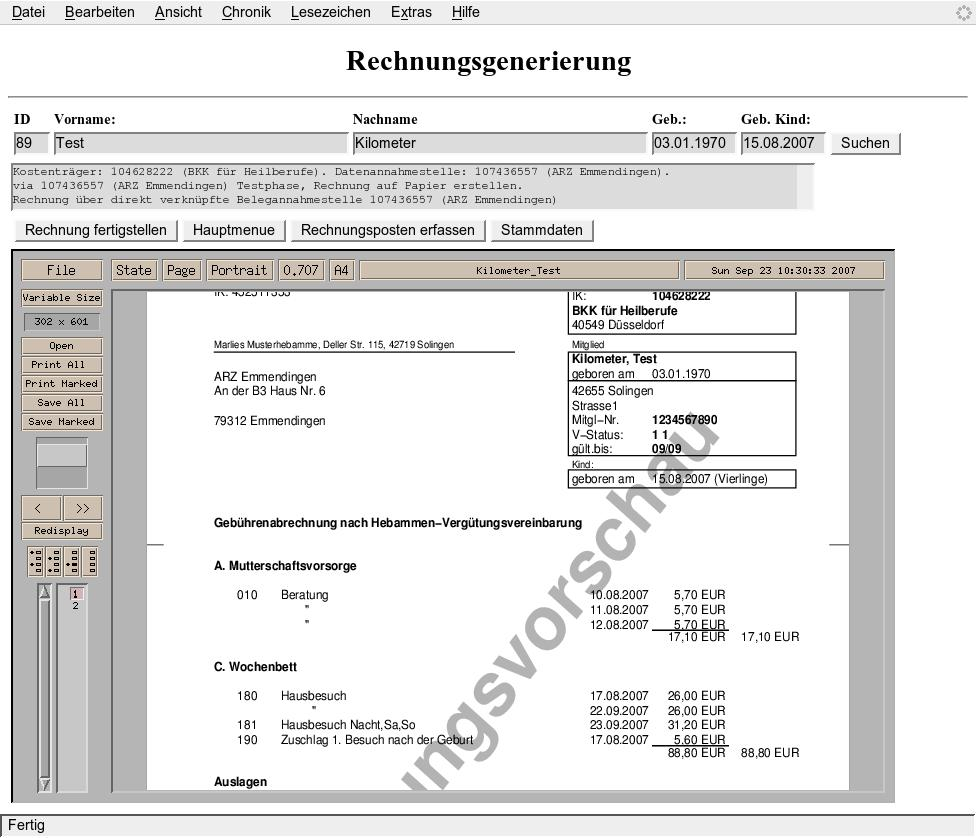
\includegraphics[width=9cm]{rechnungsgenerierung}
\caption{Rechnungsgenerierung\label{rechnungsgenerierung:fig}}
\end{figure}

Wie schon in der Kurzanleitung beschrieben, ist die Maske in zwei
Teile gegliedert. Im oberen Teil werden Daten zur Frau angezeigt,
die aktuell bearbeitet wird, sowie Informationen zur Krankenkasse.

\subsection{Daten zur Frau}
Zu den angezeigten Daten der Frau gehören 
die ID, Vor- und Nachname, sowie das Geburtsdatum der Frau und
des Kindes. Diese Felder können nicht erfasst werden. Soll eine andere
Frau ausgewählt werden, muss dies über den Knopf \knopf{Suchen} geschehen.
Die Beschreibung zu der Suchmaske befindet sich im Abschnitt 
\vref{frauenauswahl:abs}. Es werden keine Informationen in die Suchmaske
übernommen. Die Suche wird unmittelbar gestartet, dabei wird nur nach
den Frauen gesucht, die einen Status ungleich erledigt besitzen.

\subsection{Informationen zur Krankenkasse}
Die Informationen zur Krankenkasse werden nur dann angezeigt, wenn es
sich um eine Kassenrechnung handelt. Ist eine Frau privat versichert 
entfällt dieser Teil auf der Maske.

Zu jeder Krankenkasse werden die folgenden Informationen angezeigt:
\begin{enumerate} 
\item
welchem Kostenträger die Krankenkasse zugeordnet ist
\item
welche Datenannahmestelle die Krankenkasse, bzw. der Kostenträger nutzt.
\item
ob der elektronische Datenaustausch mit der Datenannahmestelle möglich ist.
\item
ob eine Belegannahmestelle vorhanden ist, an die die Rechnung geschickt
werden muss.
\end{enumerate}

\index{elektronische Rechnung}
Es gibt verschiedene Gründe, warum ein elektronischer Datenaustausch mit 
einer Datenannahmestelle nicht möglich ist. Entweder die Datenannahmestelle
ist noch nicht im Datenhaushalt von \tinyHeb\/ parametrisiert
(siehe dazu Kapitel \vref{datenannahmestellen:abs}) oder die 
Datenannahmestelle ist parametrisiert aber es liegt kein öffentlicher
Schlüssel der Datenannahmestelle vor (siehe dazu Kapitel \vref{anhang:pubkey}).

Ist die Datenannahmestelle parametrisiert und es liegt auch der
entsprechende Schlüssel der Datenannahmestelle vor, ist angegeben,
in welchem Status die elektronische Rechnung verschickt wird.
\begin{enumerate}
\item
\index{Testphase}
Testphase, diese Einstellung sollte nur für ``Spiel'' Rechnungen genutzt
werden oder zur Überprüfung, ob die Datennahmestelle Rechnungen
von der Rechnungsstellenden Hebamme entgegen nimmt.
\item
\index{Erprobungsphase}
Erprobungsphase, dies ist die Standardeinstellung von \tinyHeb\/ nach der
Installation der Software. In dieser Phase ist die Rechnung sowohl per
E-Mail, als auch per Papierrechnung zu verschicken. In der Regel wird man
nach drei Rechnungen zum Echtbetrieb zugelassen (siehe dazu auch
Tabelle \vref{krankenkassen302} im Anhang), wenn die Datenannahmestelle
schon den Echtbetrieb anbietet.
\item
\index{Echtbetrieb}
Echtbetrieb, nach der Zulassung zum Echtbetrieb ist es nicht mehr notwendig
Papierrechnungen an die Krankenkasse zu schicken. In der Maske wird die
Rechnungsvorschau trotzdem angezeigt, damit leicht überprüft werden kann,
ob die Inhalte der Rechnung ok sind.
\end{enumerate}

\subsection{Beschreibung Knöpfe in der Maske Rechnungsgenerierung}
Folgende Knöpfe sind in der Maske vorhanden:

\begin{description}
\item[Rechnung fertigstellen]
\index{Rechnung!drucken}
Dieser Knopf ist nur aktiv, wenn es sinnvoll ist eine Rechnung zu erstellen,
d.h. nur wenn wirklich Rechnungsposten vorhanden sind, die abgerechnet
werden könnten, ist der Knopf Aktiv.

Zunächst wird für jede Rechnung eine Rechnungsvorschau angzeigt. Dies
ist daran zu erkennen, dass Diagonal über die Rechnung der Text
Rechnungsvorschau angezeigt wird. Ist man mit dem Inhalt der Rechnung
zufrieden, kann über den Knopf \knopf{Rechnung fertigstellen} die
entgültige Rechnung produziert werden. Der Text Rechnungsvorschau
wird jetzt nicht mehr angezeigt. Alle Positionen, für die die
Rechnung gedruckt wurde, erhalten den Bearbeitungsstatus Rechnung,
eine weitere Bearbeitung dieser Positionen ist jetzt nicht mehr
möglich.\marginline{\Huge\bfseries!}%

Bevor die Rechnung entgültig fertiggestellt wird, prüft \tinyHeb\/ ob 
alle notwendigen Informationen für den Druck der Rechnung vorhanden sind.
Ohne die folgenden Informationen ist es nicht möglich, eine 
ordnungsgemäße Rechnung an eine Krankenkasse zu stellen:

IK Nummer der Krankenkasse, Vor- und Nachname der Frau, Geburtsdatum der
Frau und des Kindes (hier muss ggf. der errechnete Termin in den Stammdaten
erfasst werden), die Krankenversicherungsnummer und 
Versichertenstatus der Frau dürfen nicht fehlen.

Fehlt eine dieser Informationen wird eine Fehlermeldung ausgegeben und die
Rechnung \textbf{nicht} entgültig fertiggestellt. Es ist dann notwendig
über den Knopf \knopf{Stammdaten} erneut in die Stammdatenerfassung zu 
verzweigen um die fehlenden Informationen nachzuerfassen.

Fehlen Informationen zur Anschrift der Frau, wird eine Warnmeldung ausgegeben,
ob die Rechnung trotzdem erstellt werden soll. Man kann sich in diesem 
Fall entscheiden, ob die fehlenden Informationen nacherfasst,
oder trotzdem die Rechnung erstellt werden soll.

Wenn die Rechnung erfolgreich erstellt wurde, erscheint ein
Hinweistext, wie mit der Rechnung weiter zu verfahren ist, d.h.
Rechnung ausschließlich ausdrucken und per Post verschicken, ggf. zusätzlich
per E-Mail verschicken oder ausschließlich per E-Mail verschicken.
Dies ist Abhängig von der jeweiligen Krankenkasse.
Der Druck auf Papier kann für den Fall, das das Programm GV für die 
Anzeige genutzt wird, ober den Knopf \knopf{Print All} erfolgen.
Erfolgt die Vorschau, wie dies bei einer Windows Installation der Fall
ist über den Acrobat Reader, kann die Rechnung über das Druckersymbol
angestossen werden.
\item[Hauptmenue] 
Über diesen Knopf gelangt man in die Maske Hauptmenue.
\item[Rechnungsposten erfassen] 
Über diesen Knopf gelangt man in die Maske
zur Erfassung von Rechnungsposten. Ist eine Frau ausgewählt, werden deren
Daten in die Maske ``Rechnungsposten erfassen'' übernommen.
\item[Stammdaten]
Über diesen Knopf gelangt man in die Maske
zur Erfassung von Stammdaten. Ist eine Frau ausgewählt, werden deren
Daten in die Maske Stammdaten übernommen.
\end{description}


%\section{Verschicken der Rechnung per E-Mail}
\section{Verschicken der Rechnung per E-Mail\label{elekrechnung:kap}}
\index{Rechnung!per E-Mail}
Für das Verschicken der Rechnung per E-Mail existiert ein eigenes
Programm \textbf{xauftrag.pl}. Dieses Programm befindet sich im Verzeichnis
edifact und kann aus der Kommandozeile mit dem Befehl \verb|xauftrag.pl| gestartet
werden. Nachdem Start erscheint ein neues Fenster 
(Abbildung \vref{xauftrag:fig}).

\begin{figure}[ht]
\centering
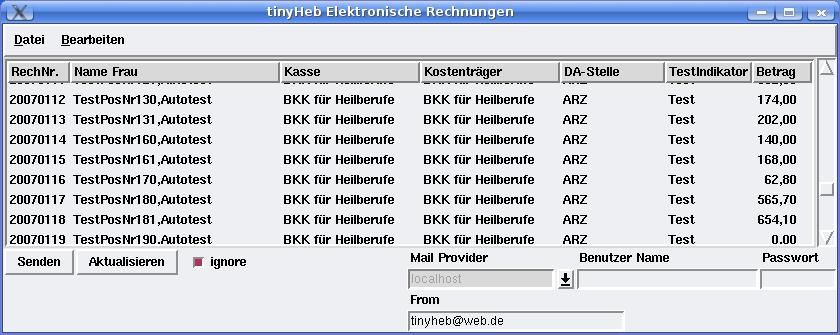
\includegraphics[width=9cm]{xauftrag}
\caption{xauftrag.pl\label{xauftrag:fig}}
\end{figure}

Das Fenster ist in zwei Bereiche geteilt. Im oberen Teil werden die
Rechnungen angezeigt, die elektronisch verschickt werden können.
Im unteren Bereich können zusätzliche Angaben gemacht werden, die bei
der Rechnungsgenerierung genutzt werden.

\subsection{Angaben zur Rechnung}
Zu den angezeigten Daten der jeweiligen Rechnung gehören die
Rechnungsnummer, Vor- und Nachname der Frau, die Krankenkasse der
Frau, der Kostenträger der Krankenkasse, die Datenannahmestelle,
Angabe des Testindikators (Test, Erprobungsphase oder Echtbetrieb)
und der Rechnungsbetrag. Es werden nur die Rechnungen angezeigt, die
noch nicht elektronisch verschickt wurden und bei denen die Möglichkeit
zum elektronischen Rechnungsversand besteht.
Eine Rechnung kann durch Anklicken zum
elektronischen Versand ausgewählt werden. Sollen mehrere Rechnungen
zum Versand ausgewählt werden, kann dies durch Halten der Taste STRG
und Klicken auf weitere Rechnungen erreicht werden. Ausgewählte
Rechnungen werden in der Farbe Blau angezeigt.

\subsection{Felder und Knöpfe}

\begin{description}
\item[Senden]
Durch Klicken auf den Knopf \knopf{Senden} werden die ausgwählten Rechnungen
an die entsprechenden Datenannahmestellen und die Hebamme (in Blindkopie)
verschickt.\footnote{ggf. 
ist es notwendig vor dem Senden eine Verbindung mit dem Internet herzustellen} 

Kann eine Rechnung erfolgreich verschickt werden, wird ein neues Fenster
geöffnet, in dem dies angezeigt wird. Das Fenster muss durch Klicken
auf den Knopf \knopf{OK} geschlossen werden, bevor weitere Rechnungen
verschickt werden können. Die Rechnung erhält den Status 
``Edi Rech'', für elektronische Rechnung und wird aus der Übersicht der
Rechnungen entfernt.

Tritt ein Fehler beim Verschicken der Rechnung auf, wird ein neues Fenster
geöffnet, in dem eine entsprechende Fehlermeldung angezeigt wird. Das
Versenden der Rechnungen wird abgebrochen und das Fenster muss
durch Klicken auf den Knopf \knopf{OK} geschlossen werden. 
Mögliche Ursachen für einen
Fehler sind z.B. eine fehlende Verbindung zum Internet (Fehlermeldung:
``The SMTP server mail.web.de was not found'') oder ein falsches
Passwort für die Anmeldung beim Provider (Fehlermeldung: ``Login not
accepted'').

\item[Aktualisieren]
Durch Klicken auf den Knopf \knopf{Aktualisieren} wird der Datenbestand
von \tinyHeb\/ auf alle Rechnungen durchsucht, die elektronisch verschickt
werden können. Diese Rechnungen werden angezeigt. Dies ist dann von
Interesse, wenn man weitere Rechnungen wie in Kapitel 
\vref{rechnungsgenerierung:kap} beschrieben, fertiggestellt hat 
und diese verschicken
möchte ohne das Programm xauftrag.pl neu zu starten.

\item[ignore]
\index{Rechnung!erneut elektronisch verschicken}
Wird das Feld \feld{ignore} angewählt und zusätzlich der Knopf
\knopf{Aktualisieren} gedrückt, werden alle Rechnungen angezeigt,
bei denen die Möglichkeit besteht, diese elektronisch zu versenden.
Dies ist unabhängig vom Status der Rechnung, d.h. es werden auch solche
Rechnungen angezeigt, die schon elektronisch verschickt wurden.
Rechnungen die schon beglichen sind, werden nicht angezeigt.
So ist es möglich einzelne Rechnungen mehr als einmal zu versenden,
falls es zu Problemen beim Rechnungsversand gekommen 
ist.\footnote{dies sollte in der Regel nicht notwendig sein}

\item[Mail Provider]
\index{Mail Provider}
\index{Internet Provider}
\index{T-Online|see{Mail Provider}}
\index{Arcor|see{Mail Provider}}
\index{Web.de|see{Mail Provider}}
\index{Freenet|see{Mail Provider}}
Über dieses Pop-Down-Menue kann der benötigte E-Mail Provider ausgewählt
werden. Als Standard Mail Provider ist auf Unix-/ Linux Systemen localhost 
angegeben, 
da \tinyHeb\/ davon ausgeht, das ein 
eigener MTA\footnote{Mail Transfer Agent} bei einer Linux
Installation üblich ist. Auf Windows Systemen wird der erste Provider,
der in der Datei \verb|.xauftragrc| angegeben ist vorgeblendet (siehe
dazu Kapitel \vref{anhang:provider}).
Sobald ein Mail Provider ausgewählt wurde, werden die Felder
\feld{Benutzer Name, Passwort} und \feld{From} gefüllt. Woher diese
Informationen kommen und wie zusätzliche Provider hinterlegt werden
können ist im Anhang in Kapitel \vref{anhang:provider} beschrieben.

\item[Benutzer Name]
Dieses Feld enthält den Benutzer Namen, der benötigt wird, um sich bei
seinem Provider anzumelden. Wird kein Benutzer Name für die Anmeldung
benötigt, kann das Feld leer bleiben.

\item[Passwort]
Dieses Feld enthält das Passwort, welches benötigt wird, um sich bei seinem
Provider anzumelden. Wird kein Passwort benötigt, kann das Feld leer
bleiben.

\item[From]
Dieses Feld wird in die From Zeile der E-Mail übernommen und muss
zwingend das Format name@provider.de haben. Die Datenannahmestellen
schicken die Bestätigung, ob die Rechnung empfangen wurde, an diese
E-Mail Adresse.
\end{description}

\subsection{automatische E-Mail Antwort der Datennahmestelle}
Je nach Verarbeitungsgeschwindigkeit
der Datenannahmestelle bekommt man nach ca 15 Minuten bis zu 3 Stunden eine
Rückmeldung von der Datenannahmestelle per E-Mail, ob die Rechnung
verarbeitet werden konnte oder ein Fehler aufgetreten ist.

Sollte nach einem Tag noch keine Antwort von der Datenannahmestelle 
eigentroffen, kann dies unterschiedliche Ursachen haben, folgende Ursachen
sind bisher Evident geworden:
\begin{enumerate}
\item 
\index{Spam}
Man hat bei seinem E-Mail Provider einen Spam-Filter eingerichtet.
Die Antwort der Datennahmestelle wird als Spam Mail erkannt.
Für diesen Fall muss der Spam Filter angepasst werden.
\item
\index{DDG}
Die Datennahmestelle ist nicht mit der Rechnungsprüfung von der
Krankenkasse beauftragt, obwohl dies in der Kostenträgerdatei so hinterlegt
ist. Dies tritt insbesondere bei der Datennahmestelle DDG auf. Da die DDG
aber b.a.w. keinen Echtbetrieb anbieten wird ist dies nicht schlimm und
man  wird über den Sachverhalt schriftlich per Brief hingewiesen.
Eine Anpassung der Krankenkassendaten ist in diesem Fall notwendig.
\item 
Die Datennahmestelle erkennt die elektronische Rechnung als Spam und
verarbeitet die Rechnung nicht. Dies ist insbesondere beim ARZ-Emmendingen
der Fall, wenn die Rechnung über den E-Mail Provider Arcor verschickt wird.
Für diesen Fall hilft es nur, sich einen neuen E-Mail Provider zu suchen,
da weder Arcor noch das ARZ-Emmendingen bereit sind, Änderungen ihrer
Einstellungen vorzunehmen.
In \tinyHeb\/ besteht die Möglichkeit Rechnungen über unterschiedliche
Provider zur verschicken, welche Einstellung dazu vorzunehmen sind, ist
im Anhang in Abschnitt \vref{anhang:provider} beschrieben. Siehe dazu
auch die Beschreibung des Feldes \feld{Mail Provider} weiter oben.
\item
\index{Signatur}
Die Rechnung wurde nicht mit einer elektronischen Unteschrift versehen
(Signatur), die Datenannahmestelle verlangt aber, dass die Rechnung
signiert ist. Dies ist z.B. bei Medent, Syntela und Autovision der Fall.
\end{enumerate}

\paragraph{Beispiel für eine erfolgreiche Annahmebestätigung (hier ARZ-Emmendingen)}
\begin{verbatim}
Annahmebestaetigung 451234567 TSOL0014.auf
 Datum: 01.05.2006 11:45
 Von: Team DALE <dale@arz-emmendingen.de>
 An: 451234567 <tinyheb@web.de>
 
Diese E-Mail wurde automatisch erstellt!

Sehr geehrte Damen und Herren,

wir bestaetigen ihnen den Empfang der gesendeten Nachricht.

Eine Pruefung der von ihnen gelieferten Daten fuehrte zu dem Ergebnis:
Die Nachricht entspricht dem geforderten Aufbau und kann an die 
nachgelagerten Pruefverfahren weitergegeben werden.

Die folgenden Dateien sind in das System uebernommen worden:
TSOL0014.auf 348
TSOL0014 1641

Die Verarbeitungsergebnisse aus den Pruefstufen 1 - 4 werden separat 
protokolliert. 
Im Fehlerfall erhalten Sie hierzu separate Meldungen.

Für etwaige Rueckfragen wurde die Datenlieferung unter der 
Referenznummer 451234567_20060501114501_0 registriert.

Mit freundlichen Gruessen

Team DALE

---

Abrechnungszentrum Emmendingen
Team DALE
An der B3 Haus Nr. 6
79312 Emmendingen
www.arz-emmendingen.de
\end{verbatim}

\paragraph{Beispiel für eine nicht erfolgreiche Annahmebestätigung (hier Medent)}
\begin{verbatim}
FEHLERMELDUNG - 451234567
 Datum: 01.05.2006 10:41
 Von: 661200048 <sole@datenannahme.medent.de>
 An: 451234567 <tinyheb@web.de>
 Antwort an: 661200048 <clearing@medent.de>
 
TSOL0012.auf, 348, 20060501:1041
TSOL0012, 1553, 20060501:1041


Sehr geehrte Damen und Herren,

eine Verarbeitung Ihrer Abrechnungsdaten ist nicht moeglich, da die 
gelieferten Daten Fehler beinhalten, die zu einer Abweisung fuehren.


Daten der Anlieferung:

Uebermittelt am:         01.05.2006
Datei-Name:              TSOL0012
Bearbeitungsnummer:      981868

Erstellt am (UNB):       -
Datei-Name (UNB):        -
Datei-Nr. (UNB):         -

IK-Kostentraeger:        -
IK-Rechnungssteller:     -
Rechnungsnummer:         -
Rechnungsdatum:          -

Fehlerbeschreibung:

Es sind Fehler in der Pruefstufe 1 aufgetreten.
[2183] Es ist keine verschluesselte Nutzdatendatei vorhanden, 
oder die Nutzdatendatei ist nicht lesbar 


Ihre eventuell eingehenden Verordnungen koennen wir zur Zeit aus 
vorgenanntem Grund keine Daten zuordnen. Wir pruefen bis zu 5 Tage 
nach Eingang der Verordnungen, ob wir zwischenzeitlich die 
Daten erfolgreich annehmen konnten, andernfalls muessen wir zu unserer 
Entlastung die eingegangenen Verordnungen wieder zuruecksenden. 
Bitte reichen Sie Ihre Abrechnungsunterlagen nach erfolgter Klaerung 
wieder ein.
Falls Ihren Unterlagen eine ausfuehrliche Papierrechnung 
(incl. Einzelpreise und Positionen) beiliegt, wird diese nach Ablauf 
der 5-Tagesfrist zur Rechnungspruefung verwendet und ggf. nach Auftrag 
des Kostentraegers, eine pauschale Rechnungskuerzung nach 303 SGB V 
vorgenommen.

Mit freundlichen Gruessen,

Medent GmbH

Bei Fragen wenden Sie sich bitte an unser Team Datenaustausch unter 
Tel.: 089 / 961 77 - 511.
\end{verbatim}
Die Fehlermeldung war im o.g. Beispiel ist übringens nicht auf \tinyHeb\/ 
zurückzuführen, sondern Medent war 2006 noch nicht in der Lage PKCS\#7
verschlüsselte Nutzdaten entgegenzunehmen\footnote{Bei Mednet müssen
Rechnungen verschlüsselt und signiert sein}.

\index{Rechnung!erneut elektronisch verschicken}
Ist es notwendig eine identische Rechnung ein zweitesmal zu 
verschicken --z.B. über einen anderen Mail Provider-- 
können durch einen
Klick auf \knopf{Ignore} und den Knopf \knopf{Aktualisieren} alle 
Rechnungen angezeigt werden, die noch nicht erledigt sind und bei denen 
es möglich ist, diese elektronisch zu verschicken.





\section{Rechnungsbearbeitung}\label{rechnungsbearbeitung:kap}
Wie schon in der Kurzanleitung beschrieben, ist es nach Erstellung
einer Rechnung notwendig, den
Zahlungseingang zu überwachen.
 Dazu dient die Maske Rechnungsbearbeitung. In die Maske gelangt
man aus dem Hauptmenue über den Link 
\verb|versandte| \verb|Rechnungen| \verb|bearbeiten|. 
Die Maske ist in zwei Teile
gegliedert. Im oberen Teil werden die Rechnungen angezeigt, die bisher
erstellt wurden, im unteren Teil können einzelne Rechnungen bearbeitet werden.

Welche Rechnungen angezeigt werden, lässt sich durch die Auswahlbox
\feld{Anzeige Einschränken} beeinflussen. Es sind zwei verschiedene Werte
möglich. Bei ``alle'', werden alle Rechnungen angezeigt. Bei
``ungleich erl.'' werden nur die Rechnungen angezeigt, die sich in einem
Status ungleich ``erl.'' befinden.

\begin{figure}[ht]
\centering
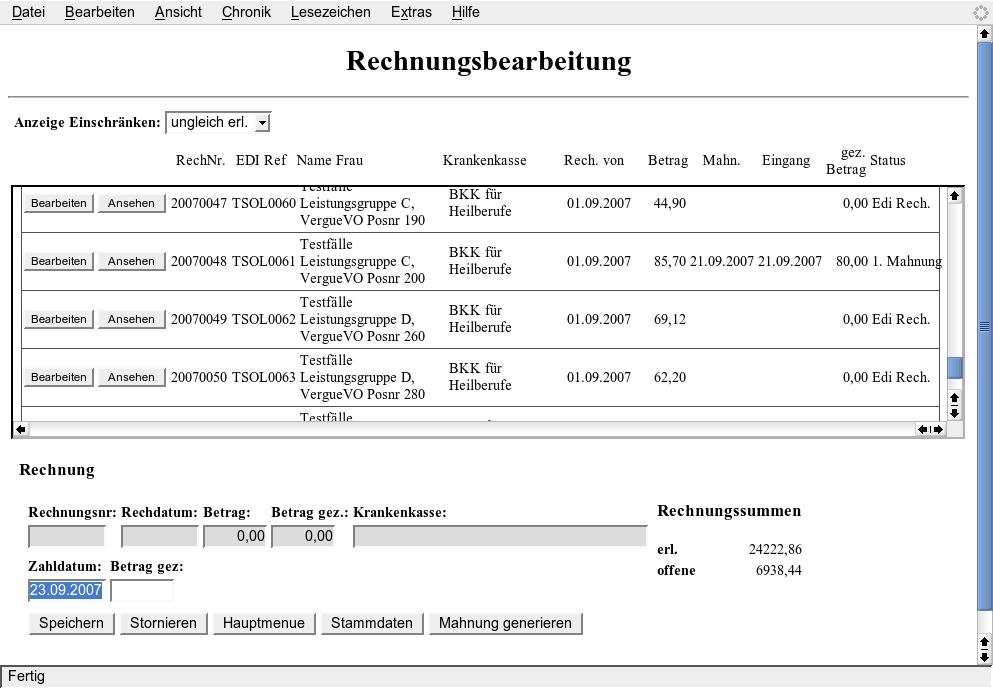
\includegraphics[width=9cm]{rechnungsbearbeitung}
\caption{Rechnungsbearbeitung\label{rechnungsbearbeitung:fig}}
\end{figure}

\subsection{Übersicht der Rechnungen}
\index{Rechnungsübersicht}
\index{ESOL}
\index{TSOL}
Zu den angezeigten Daten einer Rechnung gehören die Rechnungsnummer,
die Datenaustausch\-referenz (EDI Ref),
\index{Datenaustauschreferenz}
Vor- und Nachname sowie Krankenkasse der Frau, das Datum der Rechnungsstellung,
der Rechnungsbetrag, das letzte Mahndatum -- falls die Rechnung schon
angemahnt wurde, dass Datum des letzten Rechnungseingangs, 
der gezahlte Betrag und
der Status in dem sich die Rechnung befindet. Folgende Status sind
in der Anzeige möglich:

\begin{description}
\item[Rechnung] 
Es wurde eine Papierrechnung erstellt.
\item[Edi Rech.] 
Es wurde eine elektronische Rechnung erstellt.
\item[Teilzahl.] 
Es wurde für eine Rechnung eine Teilzahlung geleistet.
\item[Mahnung] 
Es wurde für eine Rechnung bereits eine Mahnung erstellt, 
dabei wird angegeben, wie viele Mahnung bisher erstellt wurden.
\item[Storniert]
Die Rechnung wurde storniert.
\item[erl.]
Die Rechnung wurde beglichen.
\end{description}

Neben den angezeigten Daten sind noch zwei Knöpfe in der Anzeige vorhanden.
Durch Klicken des Knopfes \knopf{Bearbeiten} wird die entsprechende
Rechnung zur Bearbeitung ausgewählt und die Daten in den unteren Teil
der Maske übernommen. Durch Klicken auf den Knopf \knopf{Ansehen} wird
ein neues Fenster geöffnet, in dem die original Rechnung angezeigt wird.
Falls die Rechnung elektronisch verschickt wurde, existiert in dem
neuen Fenster noch ein Pop-Down-Menue über das ausgewählt werden kann, ob 
die Papierrechnung oder die elektronische Rechnung angezeigt werden soll.
\index{elektronische Rechnung}

\subsection{Rechnung}
Im unteren Teil der Maske kann eine ausgewählte Rechnung bearbeitet werden.
Dies ist nur dann möglich, wenn die Rechnung noch nicht erledigt ist. Zur
Bearbeitung einer Rechnung ist es notwendig diese im oberen Teil der Maske
durch Klicken auf den Knopf \knopf{Bearbeiten}
 auszuwählen. Es kann dann im Feld \feld{Zahldatum} das
Datum des Rechnungseinganges erfasst werden und im Feld
\feld{Betrag gez:} der eingegangene Betrag. Für das Feld \feld{Zahldatum}
existieren analoge Plausiprüfungen wie für alle anderen Datumsfelder in der
Anwendung. Für das Feld \feld{Betrag gez:} wird überprüft, 
ob das Feld numerisch
mit maximal zwei Nachkommastellen erfasst wurde. Werden mehr Nachkommastellen
erfasst, wird eine Fehlermeldung ``Bitte numerischen Wert erfassen'' 
ausgegeben. Durch Klicken des Knopfes \knopf{Speichern} werden die erfassten
Werte in den Datenhaushalt übernommen, dabei ist folgendes zu beachten:

\begin{enumerate}
\item
Es wird geprüft, ob der eingegangene Betrag kleiner ist, als der ursprüngliche
Rechnungsbetrag. \tinyHeb\/ weisst auf diesen Sachverhalt hin und fragt,
ob die Rechnung trotzdem auf erledigt gesetzt werden soll. Beantwortet man
die Frage mit ``nein'', erhält die Rechnung den Status ``Teilzahlung''. 
Beantwortet man die Frage mit ``ja'', erhält die Rechnung den Status
``erledigt''.
\item
Es wird geprüft, ob der eingegangene Betrag größer ist, als der ursprüngliche
Rechnungsbetrag. \tinyHeb\/ weisst auf den Sachverhalt hin und fragt, ob die
Rechnung trotzdem gespeichert werden soll. Drückt man den Knopf
\knopf{Abbrechen}, kann man den erfassten Betrag korrigieren. Drückt man
den Knopf \knopf{OK} wird die Rechnung auf den Status ``erledigt'' gesetzt.
\item 
Der im Feld \feld{Betrag gez:} erfasste Betrag und bisher eingegangene
Zahlungen werden summiert. Ist zum Beispiel der original Rechnungsbetrag 
127 EUR und
es geht eine Zahlung von 50 EUR ein, ist 50 EUR im Feld \feld{Betrag gez:}
zu erfassen. Nach dem Speichern erhält die Rechnung den Status ``Teilzahlung''.
Geht jetzt der fehlende Rechnungsbetrag von 77 EUR ein, ist im Feld
\feld{Betrag gez:} 77 EUR zu erfassen und nicht 127 EUR.
\end{enumerate}

\paragraph{Beschreibung der Knöpfe im Menue Rechnungsbearbeitung}
\begin{description}
\item[Speichern]
Durch Klicken des Knopfes \knopf{Speichern} werden die erfassten Daten
gespeichert.
\item[Stornieren]
Durch Klicken des Knopfes \knopf{Stornieren} kann die Rechnung storniert
werden. Es werden alle Einzelposten der Rechnung auf den Status 
``in Bearbeitung'' zurückgesetzt. Die Rechnung erhält den Status storniert
und kann nicht mehr bearbeitet werden. Es können nur Rechnungen storniert
werden, bei denen noch keine Zahlung erfolgt ist.
\item[Hauptmenue]
Durch Klicken des Knopf \knopf{Hauptmenue} gelangt man in das Hauptmenue.
\item[Stammdaten]
Durch Klicken des Knopfes \knopf{Stammdaten} gelangt man in die Maske zur
Erfassung der Stammdaten. War vorher eine Rechnung zur Bearbeitung
ausgewählt, werden die entsprechenden Daten der Frau sofort in der
Stammdatenmaske angezeigt. War keine Rechnung zur Bearbeitung ausgewählt,
wird die Maske leer angezeigt.
\item[Mahnung]
Durch Klicken des Knopfes \knopf{Mahnung} gelangt man in die Maske zur
Generierung von Mahnungen. Dazu ist es notwendig vorher eine Rechnung
zur Bearbeitung auszuwählen.
\end{description}



\section{Mahnungsgenerierung}\label{mahnungsgenerierung:kap}
\index{Mahnung}

In diesem Kapitel wird beschrieben, wie eine Mahnung generiert werden 
kann. In die Maske Mahnungsgenerierung gelangt man aus der Maske 
Rechnungsbearbeitung (siehe \vref{rechnungsbearbeitung:kap}) indem man dort
eine Rechnung zur Bearbeitung auswählt und auf den Knopf 
\knopf{Mahnung generieren} drückt.

Die Maske ist in zwei Teile gegliedert. Im oberen Teil werden Daten zur Frau
angezeigt, die aktuell bearbeitet wird, sowie Informationen zur Krankenkasse.

\paragraph{Daten zur Frau}
Zu den angezeigten Daten der Frau gehören 
die ID, Vor- und Nachname, sowie das Geburtsdatum der Frau und
des Kindes. 


\paragraph{Informationen zur Krankenkasse}
Die Informationen zur Krankenkasse werden nur dann angezeigt, wenn es
sich um eine Kassenrechnung handelt. Ist eine Frau privat versichert 
entfällt dieser Teil auf der Maske.

Zu jeder Krankenkasse wird angezeigt ob eine Belegannahmestelle vorhanden ist,
an die die Rechnung geschickt wird.


\subsection{Beschreibung Knöpfe in der Maske Mahnungsgenerierung}
Folgende Knöpfe sind in der Maske vorhanden:

\begin{description}
\item[Mahnung fertigstellen]
\index{Mahnung}

Zunächst wird für jede Mahnung eine Vorschau angzeigt. Dies
ist daran zu erkennen, dass Diagonal über der Mahnung der Text
Mahnungsvorschau angezeigt wird. Will man die Mahnung wirklich generieren,
kann über den Knopf \knopf{Mahnung fertigstellen} die
entgültige Mahnung produziert werden. 
Der Text Mahnungsvorschau wird jetzt nicht mehr angezeigt. 
Alle Positionen, für die die
Mahnung gedruckt wurde, erhalten den Bearbeitungsstatus n-te Mahnung.

\item[Hauptmenue]
Über diesen Knopf gelangt man sofort in das \tinyHeb\/ Hauptmenue.

\item[Rechnungsbearbeitung]
Über diesen Knopf gelangt man in die Maske Rechnungsbearbeitung.

\item[Stammdaten]
Über diesen Knopf gelangt man in die Maske Stammdaten. Die Frau mit der
entsprechenden ID wird sofort zur Bearbeitung ausgewählt.
\end{description}
